\documentclass[letterpaper,12pt,titlepage,oneside,final]{book}

\newcommand{\package}[1]{\textbf{#1}} % package names in bold text
\newcommand{\cmmd}[1]{\textbackslash\texttt{#1}} % command name in tt font 
\newcommand{\href}[1]{#1} % does nothing, but defines the command so the 

% This package allows if-then-else control structures.
\usepackage{ifthen}
\newboolean{PrintVersion}
\setboolean{PrintVersion}{false}
% CHANGE THIS VALUE TO "true" as necessary, to improve printed results for hard copies by overriding some options of the hyperref package, called below.

%\usepackage{nomencl} % For a nomenclature (optional; available from ctan.org)
\usepackage{amsmath,amssymb,amstext} % Lots of math symbols and environments
\usepackage[pdftex]{graphicx} % For including graphics N.B. pdftex graphics driver 


% Packages added for Kirsten's dissertation
\usepackage{geometry}
\usepackage{epigraph}
\usepackage{setspace}
\usepackage{xcolor}
\usepackage{epstopdf}
\usepackage {verbatim} 

\DeclareGraphicsRule{.tif}{png}{.png}{`convert #1 `dirname #1`/`basename #1 .tif`.png}
\usepackage{tikz}
\usetikzlibrary{shadings, shadows, shapes, arrows, calc, positioning, shapes.geometric}

% N.B. HYPERREF MUST BE THE LAST PACKAGE LOADED; ADD ADDITIONAL PKGS ABOVE
\usepackage[pdftex,pagebackref=false]{hyperref} % with basic options
%\usepackage[pdftex,pagebackref=true]{hyperref}
		% N.B. pagebackref=true provides links back from the References to the body text. This can cause trouble for printing.
\hypersetup{
    plainpages=false,       % needed if Roman numbers in frontpages
    unicode=false,          % non-Latin characters in Acrobat’s bookmarks
    pdftoolbar=true,        % show Acrobat’s toolbar?
    pdfmenubar=true,        % show Acrobat’s menu?
    pdffitwindow=false,     % window fit to page when opened
    pdfstartview={FitH},    % fits the width of the page to the window
    pdfnewwindow=true,      % links in new window
    colorlinks=true,        % false: boxed links; true: colored links
    linkcolor=blue,         % color of internal links
    citecolor=green,        % color of links to bibliography
    filecolor=magenta,      % color of file links
    urlcolor=cyan           % color of external links
}
\ifthenelse{\boolean{PrintVersion}}{   % for improved print quality, change some hyperref options
\hypersetup{	% override some previously defined hyperref options
%    colorlinks,%
    citecolor=black,%
    filecolor=black,%
    linkcolor=black,%
    urlcolor=black}
}{} % end of ifthenelse (no else)

\usepackage[automake,toc,abbreviations]{glossaries-extra}

\setlength{\marginparwidth}{0pt} 
\setlength{\marginparsep}{0pt}
\setlength{\evensidemargin}{0.125in} 
\setlength{\oddsidemargin}{0.125in} 
\setlength{\textwidth}{6.375in} 
\raggedbottom
\setlength{\parskip}{\medskipamount}
\renewcommand{\baselinestretch}{1}
\let\origdoublepage\cleardoublepage
\newcommand{\clearemptydoublepage}{%
  \clearpage{\pagestyle{empty}\origdoublepage}}
\let\cleardoublepage\clearemptydoublepage
% Main glossary entries---definitions of relevant terminology

% \newglossaryentry{}
% {
% name=,
% description={}
% }
% \newglossaryentry{}
% {
% name=,
% description={}
% }
% \newglossaryentry{}
% {
% name=,
% description={}
% }
% \newglossaryentry{}
% {
% name=,
% description={}
% }

\newglossaryentry{margin}
{
name=margin,
description={edge or boundary. In economics the term has an expanded metaphorically supported technical usage. Ricardo referred to the \gls{extensive margin} as the geographical limit of production and emphasised that that limit was the limit of profitable cultivation. It was where a sensible person would stop expanding the area of cultivation for economic reasons. Later economists extended the notion to the stopping point for all kinds of decisions. Using calculus they identified the conditions under which going farther adding more const more than it added.  Margin   appeared as a metaphor in the adjective  \gls{marginal} and in compound terms like \gls{marginal product}, where it refers to the effect of a small change on some variable  such as a small increase in output  from a small increase fertilizer or labour employed. Focus on such quantities is the main feature of the \gls{marginalist} approach. }
}

\newglossaryentry{consumer surplus}
{
name=consumer surplus,
description={}
}

\newglossaryentry{excess profits}
{
name=excess profits,
description={}
}

\newglossaryentry{free entry}
{
name=free entry,
description={}
}

\newglossaryentry{the second circuit of capital}
{
name=the second circuit of capital,
description={}
}

\newglossaryentry{producer surplus}
{
name=producer surplus,
description={}
}

\newglossaryentry{marginalism}
{
name=marginalism,
description={see \gls{marginalist}}
}

\newglossaryentry{produit net}
{
name=produit net,
description={Profit from a sale after having deducted the costs and charges related to the manufacture and marketing of a product.}
}

\newglossaryentry{competitive}
{
name=competitive,
description={See \gls{perfect competition}.}
}

\newglossaryentry{commodity}
{
name=commodity,
description={1) Any product  made for exchange on the market; 2) a basic good used in commerce that is interchangeable with other goods of the same type, usually  as inputs to the production of other goods or services; 3) raw materials or primary agricultural products.}
}

\newglossaryentry{marginalist}
{
name=marginalist,
description={A style of economic analysis that emphasizes marginal values as opposed to total values or average values. The significance of the distinction lies in the fact maximizing a function like the profit function or utility gives rise to expression in terms of marginal quantities like marginal cost, marginal revenue, and marginal utility. It is then possible to say a person wishing to maximize their profit or utility should want to satisfy the derived conditions on marginal values (prescription). Another step allows economists to assume that those conditions are likely to be satisfied (description). The style of argument generally relies on the use of calculus. The systematic shift to marginalist analysis is seen as the dividing line between classical and modern economics.}
}

\newglossaryentry{profit}
{
name=profit,
description={The amount retained from sale of a product after all costs including the normal cost of capital  been paid. This amount is the income of the enterprise. The normal cost of capital is thought of a price paid to the investors who lent their capital to the enterprise and must be paid as  much for its use as they would have received if they had lent to another project. }
}

\newglossaryentry{surplus value}
{
name=surplus value,
description={See \gls{surplus} and \dots value?}
}

\newglossaryentry{pseudo-rent}
{
name=pseudo-rent,
description={A term for profits used by Alfred Marshall to emphasize that profits are a form of rent, but differ in being subject to competitions  because capital, unlike land, is a produced input and is therefor only scarce in the short term. }
}

\newglossaryentry{scarcity}
{
name=scarcity,
description={}
}

\newglossaryentry{spatial rent}
{
name=spatial rent,
description={ See \gls{locational rent}}
}

\newglossaryentry{quasi-rent}
{
name=quasi-rent,
description={}
}

\newglossaryentry{Henry George Theorem}
{
name=Henry George Theorem,
description={A proof by Arnott and Stiglitz \cite{arnottAggregateLandRents1979} of the proposition that  that if economic activity is efficiently organized over a "large" space, aggregate land rents equal the aggregate losses from the decreasing returns to scale activities. In other words, consistent with the assertions of Henry George, under certain circumstances the \gls{single tax} would finance all the infrastructure costs of a city. }
}

\newglossaryentry{ground rents}
{
name=ground rents,
description={ all economic value accruing to owners of land, regardless of whether payments are explicitly made or the rents are imputed.}
}

\newglossaryentry{single tax}
{
name=single tax,
description={a tax on land and resources that Henry George and his followers suggest is capable of replacing all other taxes since, if properly implemented,it would capture all resource rents. }
}

\newglossaryentry{digitization}
{
name=digitization,
description={The process. of converting stored information to digital form or the processof replacing human mental and physical actions with digital processing and digitally directed actions. }
}

\newglossaryentry{market}
{
name=market,
description={a means by which the exchange of goods and services takes place as a result of buyers and sellers being in contact with one another, either directly or through mediating agents or institutions.}%Britannica
}

\newglossaryentry{landowner}
{
name=landowner,
description={the class of people who receive income from their ownership of land. Usually reserved for those who receive all or most of their income from land ownership and who do not work their land themselves.}
}

\newglossaryentry{working class}
{
name=working class,
description={In Classical and Marxist theory, the category of people who had only their labour to sell were called working class}
}


\newglossaryentry{petite bourgeoisie}
{
name=petty bourgeoisie,
description={a French term that refers to a social class composed of semi-autonomous peasants and small-scale merchants. They are characterized by their ownership of small amounts of productive capital - land or property and equipment.}
}

\newglossaryentry{classical rent}
{
name=classical rent,
description={This term is sometimes used to refer to Ricardos definition of rent ans the value of the original newt productivity of land, as distinct from rental price for a property or the more general notion of economic rent. See \gls{classical rent theory}, or \gls{economic rent}.}
}

\newglossaryentry{economic rent}
{
name=economic rent,
description={is any payment to the owner of a factor of production in excess of the cost needed to bring that factor into production. In classical economics, economic rent is any payment  or benefit received for non-produced inputs such as location  and through creating official privilege over natural opportunities. See \gls{rent}}
}

\newglossaryentry{locational rent}
{
name=locational rent,
description={Income or payment for the use of location. Locational value is largely created by access to people not by landowners, hence any payment for locational advantages is a rent. See \gls{rent} or \gls{land rent}.}
}

\newglossaryentry{land rent}
{
name=land rent,
description={Ricardo payment for  the natural productivity of the land, but also considered proximity to markets (locational advantages) as a source of rent. }
}

\newglossaryentry{intensive margin}
{
name=intensive margin,
description={Distinguished from the \gls{extensive margin}, which is a locational concept. Intensive refers to  enhancing the productivity of  the land by adding labour, fertilizers or other inputs, i.e. by intensifying cultivation efforts.  The intensive margin refers to the maximum intensity of additional factors of production that makes sense economically. }
}

\newglossaryentry{extensive margin}
{
name=extensive margin,
description={A term from Ricardian rent theory that refers to either land at the greatest distance from the market or land that has the minimum fertility that justifies bringing them into commercial production. A feature of land at the margin is that it generates no \gls{economic rent}. }
}

\newglossaryentry{generalized arithmetic mean}
{
name=generalized arithmetic mean,
description={ a family of functions for aggregating sets of numbers. One special case is the geometric mean,  and the Cobb-Douglas function is a special case of that. Wikipedia provides a \href{https://en.wikipedia.org/wiki/Generalized_mean}{useful discussion}. }
}

\newglossaryentry{transmission mechanism}
{
name=transmission mechanism,
description={A general term to describe the sequence of processes through which an action at one point in a system  affects a variable at another point in the system. It is commonly used when discussing  monetary policy and how  expanding the money supply eventually affects employment.}
}

\newglossaryentry{real asset}
{
name=real asset,
description={Real assets are physical assets that have an intrinsic worth due to their substance and properties. Real assets include precious metals, commodities, real estate, land, equipment, and natural resources. }
}

% % Do we want to just make this feedback loop and feedback cycle and make uses in glossary consistent?

\newglossaryentry{feedback}
{
name=feedback,
description={The result of a causal loop. A term used in cybernetics and systems theory referring to a situation in which a change in one variable affects a second variable that then affects the first one.}
}

\newglossaryentry{surplus}
{
name=surplus,
description={Any amount or production or value in excess of what  is needed to pay for all the required inputs. Profit or rent. }
}

\newglossaryentry{Ricardian rent theory}
{
name=Ricardian rent theory,
description={The version of classical rent theory propounded by David Ricardo in his essay on the corn laws and generally seen as the  canonical version of land rent theory.}
}

\newglossaryentry{land market}
{
name=land market,
description={The entire complex of institutions, agents, and rules involved in transferring ownership of land. A land market exists wherever it is possible to exchange rights in land for agreed amounts of money or services rendered.}
}

\newglossaryentry{Alonso-Jacobs cycle}
{
name=Alonso-Jacobs cycle,
description={A positive \gls{feedback} cycle that occurs when city population is increasing in the wage, as in the Alonso model, where the wage is increasing in city population, as implied by the Jacobs component of the \gls{Alonso-Jacobs model}.}
}

\newglossaryentry{Public-Private Partnerships}
{
name=Public-Private Partnerships,
description={A long-term arrangement between a government and private sector institutions, often  employed for building, equipping, operating and maintaining schools, hospitals, transport, water, and sewerage systems. PPPs are used for projects with high social but low private returns when government is unwillling or unable to provide the up-front capital cost. The private rate of return is often subsidized by a guarantee that the private investor will receive a share of the social return over the course of the project's operation.}
}

\newglossaryentry{rent-seeking}
{
name=rent-seeking,
description={An economic concept that refers to the activity, seeking to gain wealth without contributing to productivity. Gordon Tullock, who introduced  the term, identified it as a form of theft\cite{tullockWelfareCostsTariffs1967}.  %Rent-seeking is the act of growing one's existing wealth without creating new wealth by manipulating the social or political environment. 
\Gls{rent-seeking} activities have negative effects on the rest of society. They result in reduced economic efficiency through misallocation of resources, reduced wealth creation, lost government revenue, heightened income inequality.}
}

\newglossaryentry{middle class}
{
name=middle class,
description={A broad and fuzzy term used by sociologists to describe the members of the working classes who have equity and a standard of living above the subsistence level. The OECD includes anyone who earns between 75 per cent and 200 percent of median household income after tax. Based on the most recent data available from Statistics Canada, in this country that means anywhere from about \$45,000 to \$120,000. The middle class is usually defined in terms of income level. The middle class defined this way, once the economic stratum of a clear majority of North American adults, has steadily contracted in the past five decades according to
Rakesh Kochhar and  Stella Sechopoulos of the \href{https://www.pewresearch.org/fact-tank/2022/04/20/how-the-american-middle-class-has-changed-in-the-past-five-decades/}{Pew Research Centre}  in 2022.}
}

\newglossaryentry{rentier}
{
name=rentier,
description={A person living on income from property or investments rather than from current income. The term is from the  French \textit{rentier}, ``holder of rental properties or investments that pay income,'' from \textit{rente} ``profit, income'' \cite{GET_rentier_defn_quote}. %``Financial engineering has created a rentier class, a modern feudal system, and the biggest beneficiaries of all that extra debt have been the bankers.'' Times, Sunday Times (2016) 
}
}

\newglossaryentry{rate of return}
{
name=rate of return,
description={or return on investment: the money made or lost on an investment over some period of time. Expressed nominally as the change in dollar value of an investment over time or  as a percentage derived from the ratio of profit to investment. We compute the nominal return, convert it to a percentage and compare that to the investor's best alternative return or required return.}
}

\newglossaryentry{joint-stock company}
{
name=joint-stock company,
description={A joint-stock company is a business owned by its investors, with each investor owning a share of the company based on the amount that they've invested. It is a predecessor to the modern-day corporation and other types of registered companies. A joint-stock company is an artificial person; it has legal existence separate from persons composing it. It can sue and can be sued in its own name. The shareholders are usually not liable for any of the company debts that extend beyond the company's ability to pay up to the amount of them.}
}

\newglossaryentry{REIT}
{
name=REIT,
description={Real Estate Investment Trust. A REIT is a financial instrument that  makes it possible for individual investors to earn dividends from real estate investments without having to buy, manage, or finance properties themselves. Structured as a company that owns and sometimes operates income-producing real estate or related assets, REITs are modeled after mutual funds \cite[GET-reit-like-mortgages].} %cite REITs are modeled after mutual funds? 
}

\newglossaryentry{financial instrument}
{
name=financial instrument,
description={A financial instrument is a monetary contract, which confers a right or claim against some counterparty in the form of a payment (checks, bearer instruments), equity ownership or dividends (stocks), debt (bonds, loans, deposit accounts), currency (foreign exchange or forex), or derivatives (futures, forwards, options, and swaps). There are %\href{https://www.investopedia.com/terms/f/financialinstrument.asp}{many types} 
many types of financial instrument \cite[WEB-investment-types].}
}

\newglossaryentry{compound interest rate}
{
name=compound interest rate,
description={Where an interest rate is specified for a single term, such as a year, the rate for a longer, multi-period term is larger. If the calculation for a later period includes interest on the interest from earlier periods, the interest is said to ``compound.'' This is how interest is usually charged. Compound interest for a given period is calculated by multiplying the initial principal amount by one plus the annual interest rate raised to the number of compound periods minus one.}
}

\newglossaryentry{amortize}
{
name=amortize,
description={to reduce an amount gradually by making payment in installments: a to pay off (as a loan) gradually usually by periodic payments of principal and interest. }
}

\newglossaryentry{appraised value}
{
name=appraised value,
description={an evaluation of a property's value based on a given point in time. The evaluation is performed by a professional appraiser during the mortgage origination process.}
}

\newglossaryentry{premium}
{
name=premium,
description={The difference between the base price and the price paid in a particular market or buy a particular buyer. In our model is is the difference between the wage of rural workers and the wage of urban workers required to induce workers to live in the city and incur commuting costs. See \gls{urban wage},\gls{urban wage premium}, \gls{rent premium}.}
}

\newglossaryentry{subsistence frontier}
{
name=subsistence frontier,
description={The minimum income or lowest standard of living that can sustain people in the economy. Rather than thinking of the limit as a single value---say the minimum survival income---it is more realistic to recognize that the limit can be achieved with different combinations of goods. For example, if clean water is freely available in a local stream, the subsistence income does not include the cost of bottled water. All the combinations can be seen as a \gls{frontier}. \newline In classical economics, the frontier was summarized as a subsistence wage. Subsistence theorists like Malthus argued that the market price of labour would not vary from the natural price for long: if wages rose above subsistence, the number of workers would increase and bring the wage rates down. The classical economist recognized that the limit was in part set by social convention, but it was analytically convenient to assume a subsistence wage, and it could be argued, following Malthus that a subsistence wage  represented a long-term limit or \gls{equilibrium}. As an analytical convenience in our model, we employ a subsistence wage that includes housing and a conventional standard of living.  }
}

\newglossaryentry{political economy}
{
name=political economy,
description={Political economy is a branch of social science that studies the relationship  between government and the economy. As a discipline, it dates back the  16$^{th}$ but is usually associated with the political economists of the mid-18$^{th}$ and  early 19$^{th}$  century like Adam Smith who began to explore the economic implications of free markets and industrialization. Departments of political economy persisted well into the mid 20$^{th}$ C before splitting into separate departments of economics politics \cite{helleiner20PoliticalEconomy2018}.}
}

\newglossaryentry{expected market price}
{
name=expected market price,
description={The price is expected to emerge in a \gls{market} at a future point in time as a result of the interaction of buyers and sellers. It may vary as the mixture of buyers and sellers changes or as their information changes.}
}

\newglossaryentry{market price}
{
name=market price,
description={The price that emerges in a \gls{market} as a result of the interaction of buyers and sellers. It may vary as the mixture of buyers and sellers changes or as their information changes.}
}

\newglossaryentry{expectation}
{
name=expectation,
description={in our model, an agent's estimate of an unobserved or future value of a variable such as price. In simple statistical analysis the expectation of a variable may be taken as the average of the previously observed values.  }
}

% \newglossaryentry{perfect}
% {
% name=perfect,
% description={}
% }

\newglossaryentry{total factor productivity}
{
name=total factor productivity,
description={total-factor productivity (TFP), also called multi-factor productivity, is usually measured as the ratio of aggregate output  to aggregate inputs. It is a scale factor used to explain why the same combination of inputs produces different quantities of output at different places or times. It appears the factor  $A$ discussed in Chapter~\ref{chapter-growth} and in cities is influenced by the size of the population.  }
}

\newglossaryentry{factor of production}
{
name=factor of production,
description={(such as labour, land, financial capital,  and human capital)}
}

\newglossaryentry{perfect competition}
{
name= perfect competition,
description={An imaginary but analytically useful ideal market condition with the following  characteristics: 1. Large numbers of buyers and sellers in each market so that no individual buyer or seller can affect the price. 2. Free entry and exit of firms in the market. 3. Firms in each market sell a homogeneous product. 4. Buyers and sellers possess complete knowledge of the market. 5. No price controls.\newline  Economists often compare the markets they study to the` idealized, perfectly competitive market structure.}
}

\newglossaryentry{frontier}
{
name=frontier,
description={In mathematical economics, the limit of what is possible. Like the frontier of a country, even if you can't cross it, you can move along it to find the best location  subject to that constraint. In elementary economics, the budget-line and the production possibilities frontier (PPF) are  frontiers. Tf you spend less than the budget are operating inside the PPF, you could do better. Your solution is inefficient. }
}

\newglossaryentry{attractor}
{
name=attractor,
description={In \gls{dynamical system} theory as described by difference or differential equations, an attractor is a point or orbit inside a region of the phase space. The phase space is a representation of all possible states of the system each corresponding to a unique point in the phase space. If there is an attractor in the region, if the system starts at any point in the region,  it will eventually evolve to the attractor.}
}

\newglossaryentry{dynamical system}
{
name=dynamical system,
description={any system that changes over time. Typically we mean a  system that is described by a set of interrelated equations, one of which is time-dependent. }
}

\newglossaryentry{agent-based}
{
name=agent-based,
description={a term for a model that is a  collection of autonomous decision-making entities called agents. In practice the agents are little sub-programs (automata, robots) that each separately use some information about their environment and follow some internal rules to choose a response in each model cycle. See \gls{agent-based model}}
}

\newglossaryentry{price formation}
{
name=price formation,
description={The process of selecting a price based on the conditions in a system. The classic problem is the simple supply and demand model, in which sellers and buyers, each group with its own wants represented by an equation, interact to find a a price. The model  identifies a combination of price and quantity that would be acceptable to both at the same time, but doesn't say how they get to the price. It lacks a price formation mechanism.  \newline The fundamental problem is that the agents don't have complete information and may have limited computational ability, especially with multiple interacting markets. A theory of price formation has to describe the process of adjustment. This is usually represented as a set of individual adjustment rules, which makes any theory of price formation a dynamical system It may not always lead to a steady state equilibrium.}
}

\newglossaryentry{classical}
{
name=classical,
description={Referring to the period of economic theorizing primarily in Britain roughly between 1750 and 1870, prior to the neoclassical period in economics. See \gls{classical economics}.   }
}

\newglossaryentry{market rent}
{
name=market rent,
description={The amount a landlord charges a tenant for the use of a property in a competitive market. }
}

\newglossaryentry{mill rate}
{
name=mill rate,
description={The municipal tax rate: the amount per \$1,000 of the assessed value of a property which will be due as property tax.}
}

\newglossaryentry{financialization}
{
name=financialization,
description={Something is financialized when a financial instrument representing it is created. The  home mortgage market was financialized when financial institutions developed markets that let let investors buy and sell mortgages between themselves. These transactions gave investors ownership of the stream of income established by the mortgage contract. The transaction did not affect the mortgage conditions or the home: they simply added a new product for investors to speculate on. }
}

\newglossaryentry{amenity}
{
name=amenity,
description={a desirable or useful feature or facility of a building or place.}
}

\newglossaryentry{population}
{
name=population,
description={In our model, the number of city residents. }
}

\newglossaryentry{financialize}
{
name=financialize,
description={Something is financialized when a financial instrument representing it is created. For example, mortgages originated in England when people did not have the resources to purchase land in one transaction. Buyers would get loans directly from the seller---no banks or outside parties were involved. Home mortgages were financialized when financial institutions developed markets that let them buy and sell mortgages between themselves.  See \gls{financialization}}
}

\newglossaryentry{housing market}
{
name=housing market,
description={A market is defined as the sum total of all the buyers and sellers engaged in the transfer of ownership of an asset, good or service, plus all of the institutional machinery that supports the transactions. }
}

\newglossaryentry{urban center}
{
name=urban center,
description={In our model the urban centre is a point at the center of a population agglomeration where all employment is located. More generally it is the area within an urban agglomeration with with the largest  concentration of employment and or commercial activities.} 
}

\newglossaryentry{functional form}
{
name=functional form,
description={the algebraic form of a relationship between a dependent variable and explanatory variables.}
}

\newglossaryentry{production}
{
name=production,
description={The process of converting a set of \glspl{input} into a desired \gls{output}. See\gls{factor of production}.}
}

\newglossaryentry{perfectly elastic}
{
name=perfectly elastic,
description={Producing more won't affect the product's price. The term describes a  horizontal supply or demand curve. See \gls{elasticity}.} % On a \gls{supply demand curve} (is that the right name?) ***}
}

\newglossaryentry{elasticity}
{
name=elasticity,
description={The ratio of the percentage change in a quantity to the percentage change in another quantity. The price elasticity of demand, for  example, would be the percentage change in the quantity demanded that accompanies a one-percent change in price. It is a (local) property of a demand curve and would typically be a negative number like $-0.3$ or $-1.5$, since demand typically slopes downward. See \gls{perfectly elastic}.}
}

\newglossaryentry{labour augmenting agglomeration}
{
name=labour augmenting agglomeration,
description={The situation in which bringing more workers together increases their average productivity.}
}

\newglossaryentry{present discounted value}
{
name=present discounted value,
description={The amount that someone should be willing to pay, in the present, for a stream of expected future payments.}
}

\newglossaryentry{wealth}
{
name=wealth,
description={In our model, wealth is the set of valuable economic resources owned, by an individual or organization as measured in either real goods or money value, that the bank considers in lending decisions. We model only housing and aggregate financial wealth (savings), but more generally, wealth includes stocks of human capital, equities, land, and other more subtle assets.}
}

\newglossaryentry{input}
{
name=input,
description={In production theory, an input is any good or service used to produce another another good or service. % anything  that is among the collections of goods and services that is used to produce a desire  product or service. 
For example, labour is a necessary input for producing food. }
}

\newglossaryentry{output}
{
name=output,
description={In production theory, an output anything produced.} % Often symbolized by $Y$ or $Q$  in relations like $Y= F(K,L,N)$.}
}

\newglossaryentry{subsistence wage}
{
name=subsistence wage,
description={In most urban models the subsistence wage is treated as base cost that is the opportunity cost of agricultural land. We have extended the technique to include the opportunity cost of urban labour. It is one of the simplifications which makes our model tractable and focuses it on the question of rents and the specifically urban productivity premium. In our model, the subsistence wage is a wage available inside and outside the urban area, which covers the cost of buildings, food, core living costs, and a base cost of land.}
}

\newglossaryentry{urban wage premium}
{
name=urban wage premium,
description={The wage premium is the premium above the \gls{subsistence wage} payed by employers to attract workers. An urban wage premium appears when workers in larger cities earn higher average wages than workers in smaller cities. In both the U.S. and Sweden a wage premium has been shown to follow a power-law relationship that scales superlinearly with city size. In other words, workers in larger cities not only earn higher average wages, they do so systematically as a power law function of the size of the city. Bettencourt  \cite{bettencourtIntroductionUrbanScience2021}, has demonstrated theoretically that a wage premium should manifest as a power law function and predicted the value of its exponent.}
}

\newglossaryentry{urban wage}
{
name=urban wage,
description={The \gls{urban wage} is the \gls{urban wage premium} plus the \gls{subsistence wage}.}
}

\newglossaryentry{product}
{
name=product,
description={A product is anything produced. It is an \gls{output} of a production process. % Our model has no specific products. 
Rather than specific products, the city in our model produces an aggregate output, which is not a variable in our analysis. Instead of producing explicit list of discrete products, output is defined by an implicit production function relating labour as an input to aggregate productivity and thus to wages. % as part of urban incomes.
}
}

\newglossaryentry{imperfect competition}
{
name=imperfect competition,
description={A market in which any of the conditions required for \gls{perfect competition} are not met.}
}



\newglossaryentry{demand function}
{
name=demand function,
description={An equation describing how much a potential buyer or group of buyers will purchase at any given price. It can express price as a function of quantity or quantity as a function of price. In either case it will usually include other variables that are said to "shift" demand.   }
}

% \newglossaryentry{supply demand curve}
% {
% name=supply demand curve,
% description={}
% }

\newglossaryentry{increasing returns to scale}
{
name=increasing returns to scale,
description={a property of a production process  such that that when all the inputs are increased in the same proportion, the quantity of \gls{output} increases by a greater proportion.}
}

\newglossaryentry{decreasing returns to scale}
{
name=decreasing returns to scale,
description={a property of a production process  such that that when all the inputs are increased in the same proportion, the quantity of \gls{output} increases by a lesser proportion.}
}

\newglossaryentry{constant returns to scale}
{
name=constant returns to scale \gls{CRS}. ***,
description={a property of a production process such that that when all
the \glspl{input}s are increased in the same proportion, the quantity of \gls{output} increases by the same proportion.  }
}

\newglossaryentry{equilibrium condition}
{
name=equilibrium condition,
description={A condition that must be satisfied if a resultant variables of the system are to remain constant. ``For an equilibrium of prices and quantities in normal free \gls{market}, supply must equal demand.''}
}

\newglossaryentry{population equilibrium}
{
name=population equilibrium,
description={an \gls{equilibrium condition} that ensures population will not rise or fall  for the region under consideration. In urban model it is the condition that people cannot make themselves better off by moving to another location in the system. Formally it can be expressed by the requirement that the utility of people with the same  assets and tastes is equal at every location. }
}

\newglossaryentry{urban labour supply}
{
name=urban labour supply,
description={in our model this is simply the urban population, but more generally it is all those in the general population willing to work at the location or occupation.}
}

\newglossaryentry{stochastic}
{
name=stochastic,
description={Having a random probability distribution or pattern that may be analyzed statistically but may not be predicted precisely. Introducing even a small amount of random nose into even one variable in a model of a deterministic system converts the model into a stochastic model.}
}

\newglossaryentry{aggregate}
{
name=aggregate,
description={Formed or calculated by the combination of many separate units or items; a total.}
}

\newglossaryentry{agglomeration economies}
{
name=agglomeration economies,
description={Economic efficiencies resulting from \gls{agglomeration effects}.}
}

\newglossaryentry{agglomeration}
{
name=agglomeration,
description={A collection of similar items in one location. A city is an agglomeration of people and generally of firms. Agglomeration may have properties that individuals do not have, giving rise to \gls{agglomeration effects} or gls{agglomeration economies}.}
}

\newglossaryentry{locational equilibrium}
{
name=locational equilibrium,
description={A situation in which no resident will make herself better off by moving to another location. A Nash equilibrium with housing efficiently allocated  given market prices. See \gls{migration equilibrium}.}
}

\newglossaryentry{agglomeration effects}
{
name=agglomeration effects,
description={An effect of increasing the number of firms  or workers in one place. A larger, deeper, more specialized labour pool enables workers to better match their skills to the needs of firms or creates knowledge spillovers in which firms and workers learn from each other.}
}

\newglossaryentry{monopolistic competition}
{
name=monopolistic competition,
description={A type of  \gls{imperfect competition}. \gls{Perfect competition} is a description of a market with many seller, all of whom are price-takers. Monopoly is a market with a single seller, who therefore has the power to set the selling price. Monopolistic competition describes cases in between, with sellers that have some power to set prices within a segment of the market. It occurs when many companies offer competing products or services that are similar, but are not perfect, substitutes.}
}

\newglossaryentry{labour adjustment cost}
{
name=labour adjustment cost,
description={Costs associated with hiring, firing or training that prevent or slow the rate at which a firm will increase or decrease the number of workers it employs.}
}

\newglossaryentry{frictional unemployment}
{
name=frictional unemployment,
description={the part of total unemployment  due to people being in the process of voluntarily moving from one job to another.}
}

\newglossaryentry{marginal product}
{
name=marginal product,
description={the amount that the last unit of any factor  adds to output while holding all other factors constant. See \gls{marginal product of labour}.}
}

% \newglossaryentry{marginal product of labour}
% {
% name=marginal product of labour,
% description={Firms calculate what the next worker is worth to them. That's what they're willing to pay for labour. 
% This is the labour \gls{demand function} based on the \gls{marginal product} which is declining. When a firm has only a few workers, it is high on that demand function, and has to move down. It cuts workers. If it's too low, it expands and hires. %This says something about the geometry of what employers could pay. 
% % Firms can't pay workers more than they can earn in the long term, unless that money comes from somewhere, but they could push down wages and extract more profit, invest more in other factors of production, etc.
% }
% }

\newglossaryentry{marginal product of labour}
{
name=marginal product of labour (MPL),
description={the amount that the last worker  adds to output without changing the quantities of other inputs used. The firm's \gls{demand function} for labour in a competitive market is identically  the \gls{marginal product} of labour function, represented as a downward sloping curve due to the diminishing marginal productivity of labour. See \gls{marginal}.}
}

\newglossaryentry{monopoly}
{
name=monopoly,
description={ Market power means you can price above marginal costs. Need free entry to get rid of it---it doesn't drive out profit---profits can be sustained over longer. Monopolist can charge a higher price but pays a competitive price for all \glspl{input} including labour. If a firm also had a monopoly on offering jobs, they could drive down wages.}
}

\newglossaryentry{duopoly}
{
name=duopoly,
description={A market with two sellers. Under one set of assumptions the result will be the monopoly price, under others, the situation will generate lower  than monopoly prices, ore even competitive pricing and may result in market instability.}
}

\newglossaryentry{monopsony}
{
name=monopsony,
description={A market with one buyer who therefore has some power to determine the purchase price by varying the quantity purchased. An example of \gls{imperfect competition}.}
}

\newglossaryentry{imperfect information}
{
name=imperfect information,
description={ the buyers and/or sellers do not have all the information necessary to make an informed decision.}
}

\newglossaryentry{externalities}
{
name=externalities,
description={any indirect costs or benefit to uninvolved third parties that are an effect of a decision-makers activity but are not included in the decision-maker's cost-benefit calculations. Lawn mowers may wake the neighour, emissions from vehicles cause emphysema, burning fossil fuels may contribute to climate change, or painting your house may raise the value of the neighbour's house. In our model, when employers increase their workforce there is a positive effect on the productivity of all other workers in the city. This is an external effect}
}

\newglossaryentry{competitive market}
{
name=competitive market,
description={**FIX Everybody is a price taker. Price takers don't assume anything they do affects other producers or suppliers, so they act in terms of their internal prices and costs. 
This means their decision making process doesn't take into account any one else's behaviour.
? The easy way to see that is assume prices are fixed - all that's required to get the behaviour \dots  have a few other things like free exit and entry, perfect information etc---to get the efficiency result.} % (or to ensure price taking)}
}

\newglossaryentry{effective labour}
{
name=effective labour,
description={FIX - Effective labour is the productive \gls{output} from labour. As soon as you introduce agglomeration economies, labour becomes a more complex phenomena. There is the benefit of the single worker which should be perfectly declining on that nice concave production function and there is the diagonal movement as a result of increasing productivity because you keep adding people to the market. That means that your productivity of the worker isn't' just attached to the worker and your plant. It has this other component \dots 'effective labour'---the output including the A term.}
}

\newglossaryentry{spillover effects}
{
name=spillover effects,
description={ \Gls{externalities} are the most commonly discussed form of spillover effects but any economic event in one context that occurs because of something else in a seemingly unrelated context can be considered a spillover. It is a looser term than externality because an externality is a consequence, at least in economic theory, of rational optimizing behaviour.}
}

\newglossaryentry{substitutable}
{
name=substitutable,
description={One good may be substituted for another without loss of benefit. Two brands of motor oil are good substitutes for each other. Oranges are somewhat subsitutable for apples , but not for screwdrivers.}
}

\newglossaryentry{neoclassical distribution theory}
{
name=neoclassical distribution theory,
description={A theory that states that in perfect competition the owner of every unit of every  \gls{factor of production} will be paid precisely the  value of the \gls{marginal product} of that factor for each unit unit they contribute to production.}
}

\newglossaryentry{Solow-Swan model}
{
name=Solow-Swan model,
description={a  model of macro-economy developed and analysed by Robert Solow and Trevor Swan independently to explain long-run economic growth \cite{dimandTrevorSwanNeoclassical2009}. It attempts to explain  growth in terms of the growth of three contributing factors, capital, labor (population),  and  productivity.}
}



\newglossaryentry{migration equilibrium}
{
name=migration equilibrium,
description={The theoretical situation in which no resident can  make themselves better off by moving to another location. It is a logical consequence of utility maximization and free mobility that results in a Pareto optimal allocation of housing. Technically it is a Nash equilibrium, While extremely useful in analysing urban systems, the concept does not closely describe real cities.
% A situation in which not resident will make herself better off by migrating to or between cities or countries. Similar to a migration equilibrium.
}
}

\newglossaryentry{commuter shed}
{
name=commuter shed,
description={For a city, the area over which people will travel to work in a city. In the \gls{Alonso-Jacobs model}, it is sharply defined by the maximum distance commuters can travel before transportation costs exceed the wage premium. In  practice, the duration of commutes is highly variable. It is greater in the case of men, singles, educated and foreign workers, persons living in rented housing, using public transport, living or working in large cities, or working in large firms,  and when the  unemployment rate is high\cite{axisaFactorsInfluencingCommute2012} .}
}

\newglossaryentry{circular city}
{
name=circular city,
description={In urban theory, an idealized city form predicted by models with uniform travel costs in all directions and a fixed household commuting budget. If a city is laid out on a rectangular grid, the same travel-cost logic yields a rectangular city. Recently the term is applied to cities committed to achieving a circular economy. }
}

\newglossaryentry{radial city}
{
name=radial city,
description={A radial concentric city plan is formed by streets that extend outward from a defined center and reach the outer edge of the city, together with concentrically arranged roads that connect the radial streets to the lots. it is an idealized pattern that traces back to ancient times and appears  today in planned cities and districts. See \gls{circular city}.}
}

% \newglossaryentry{surplus}
% {
% name=surplus,
% description={Or economic surplus. Any social product in excess of the minimum required to reproduce society. In value terms the surplus appears as profit or rent and accrues to the owner of a  scarce \gls{input} that varys in quality, such as land. In the mid-19th century, French engineer Jules Dupuit first extended the concept of economic surplus to what came to be called producer- and consumer-surplus.}
% }

\newglossaryentry{Alonso-Jacobs model}
{
name=Alonso-Jacobs model,
description={A model combining the \gls{Alonso model} of the urban land use  \cite{alonsoModelUrbanLand1960} with the \gls{agglomeration} theory of Jane Jacobs \cite{jacobsEconomyCities1969} which explains the productivity of cities.}
}

\newglossaryentry{monopsonist}
{
name=monopsonist,
description={A single buyer, usually in an input market. A monopsonist is not a price-taker, knowing that buying more well result in  higher prices. This rleads the monopsonist to purchase less than is socially efficient.}
}

\newglossaryentry{financial return}
{
name=financial return,
description={MAYBE ADD what is best definition? - there may be other returns. Assessed by comparing the net rent $\mathcal{R}_N$ to the costs of acquiring a property, in particular to the cost of borrowing money. CLARIFY}
}

\newglossaryentry{home services}
{
name=home services,
description={A property offers two kinds of services: home services and \gls{locational services}. Home services describes the value offered by living in a house: a place to sleep, to prepare food, the amenity of being in the home, etc. Since people require housing inside and outside the city, home services are modeled as paid for as a share of the subsistence wage ($a \psi$).}
}

\newglossaryentry{locational services}
{
name=locational services,
description={A property offers two kinds of services: \gls{home services} and locational services. Locational services are services accessed by right of location. They include access to the central city job, access to locational amenity, and the benefit of services and connections associated with a location. In the core model, Locational services are, on an annual basis, the rent premium $w$, minus the transportation costs $c$ for a property a given distance, $d$, from the center, $\omega- {dc}$.}
}

\newglossaryentry{rent share}
{
name=rent share,
description={}
}

\newglossaryentry{Pareto efficiency}
{
name=Pareto efficiency,
description={An economic state where resources cannot be reallocated to make one individual better off without making at least one individual worse off.}
}

\newglossaryentry{efficiency conditions}
{
name=efficiency conditions,
description={Conditions derived in neoclassical economic theory that must be satisfied if a system or activity is to achieve Pareto efficiency. Under somewhat reasonable conditions the efficiency conditions are achieved by agents acting in a decentralized manner to maximize their own profit or utility.}
}

\newglossaryentry{neoclassical economics}
{
name=neoclassical economics,
description={An approach to the study of the economy and economic behaviour that attempts to explain the production, pricing, and the consumption of goods and services through supply and demand, and to explain agent behaviour using a theory of rational agents who satisfy \gls{marginal} efficiency conditions. It integrates, within a mathematical framework, the cost-of-production theory from classical economics with a consumer demand theory based on utility maximization.}
}


\newglossaryentry{neoclassical}
{
name=neoclassical,
description={refers to a period in economic theorizing that overlaps with  but largely follows classical economics and dominates economic theory to  today. See \gls{classical economics}, \gls{neoclassical economics}.}
}

\newglossaryentry{classical economics}
{
name=classical economics,
description={Also called classical \gls{political economy}. A school of thought in political economy that flourished, primarily in Britain, in the late 18th and early-to-mid 19th century. It was part of the intellectual  development of  Western liberal democracies in the 18th and 19th centuries and  brought into the mainstream by Scottish economist Adam Smith. Its main thinkers include Adam Smith, Jean-Baptiste Say, David Ricardo, Thomas Robert Malthus, and John Stuart Mill. After 1850, key features of the classical approach were carried forward by  Karl Marx and his followers, and by Henry George. Classical economics  provided the foundation for the development of \gls{neoclassical economics}.}
}

\newglossaryentry{socioeconomic status}
{
name=socioeconomic status,
description={Socioeconomic status is typically broken into three levels, high, middle, and low,  commonly referred to as ``upper class,'' ``middle class,'' and ``working or lower class,'' it differs from `\gls{class}' in the more traditional sense, which is a functional classification. See \gls{Ricardian class}, being based on occupation, income, family wealth.}
}

\newglossaryentry{Ricardian class}
{
name=Ricardian class,
description={The conception of class in \gls{classical economics} including Marx, where class is based on the types and amounts of productive capital the individual owns. See \gls{class}.}
}

\newglossaryentry{rent profile}
{
name=rent profile,
description={see \gls{bid-rent function} or \gls{bid-rent curve}}
}

\newglossaryentry{class}
{
name=class,
description={This term has a wide range of sometimes conflicting meanings. In our usage, which is consistent with classical economics including Marx, class is based on the types and amounts of productive capital the individual owns. This is a functional definition quite distinct from socioeconomic status which is more common in the current discussion. Our treatment of the evolution of class structure with financialization draws on We allow  people in different functional classes to own financial capital, producing intermediate classes \`a la Roemer\cite{roemerGeneralTheoryExploitation1982}.}
}
\newglossaryentry{capitalize}
{
name=capitalize,
description={To capitalize a stream of expected income is to compute it's capitalized value. Capitalized value is the current worth of an asset, usually real estate, based on a calculation of present value of expected income over the course of its economic lifespan.}
}

\newglossaryentry{agglomeration effect}
{
name=agglomeration effect,
description={The external economies associated with size and concentration. The benefits of size and concentration vary for different cross-sections of the urban population. Three such groupings may be identified: 1. Consumer agglomeration economies; Business agglomeration economies; Social agglomeration economies \cite{carlinoAgglomerationEconomiesSurvey1978}.}
}

\newglossaryentry{price bubble}
{
name=price bubble,
description={The sustained rise in the price of an asset above its ``normal'' market value'' caused by agents (mainly speculators) forecasting further price increases base on previous increases, rather than on estimates on intrinsic value.  Price bubbles are sustained by expectations of future increases in the price of an asset. They may end sharply, or crash, when expectations shift.}
}

\newglossaryentry{marginal value-product}
{
name=marginal value-product,
description={Also known as the marginal revenue product. The marginal revenue created due to an addition of one unit of productive resource, such as one more worker. Calculated by multiplying the marginal physical product by the price, or the marginal revenue in the case of a non-competitive market.}
}

\newglossaryentry{neoclassical growth theory}
{
name=neoclassical growth theory,
description={An economic theory that outlines how a steady economic growth rate results from a combination of three driving forces---labour, capital, and technology. Robert Solow and Trevor Swan developed and introduced the model of long-run economic growth in 1956. It is the  foundation of most empirical and theorical attempts to explain macroeconomic growth.}
}


\newglossaryentry{capital}
{
name= capital,
description={The word "capital" has many different meanings in economics and finance.  In economics, real capital is durable produced goods that are in turn used as productive inputs. \Gls{financial capital} is wealth that can be used to lend to others in exchange for interest payments or to purchase assets. Both these forms of capital are represented in the economy by extensive legal organizational structures that represent the interests of their owners. Other forms of capital recognized by economists are human capital, social capital natural capital, and intellectual capital. The distinctive  features of capital include that it takes time and energy to create (natural capital, however is  `a free gift of nature''), lasts a long time, deprecates, produces a stream of benefits over time,  and may be transferable as property}
}

\newglossaryentry{financial capital}
{
name=financial capital,
description={Financial capital is simply lendable purchasing power. Owners of financial capital provide their liquidity to borrowers in exchange for a future return. Interest rates are the prices charged for the use of financial capital. It is generally based on (secured by) ownership of tradable assets.  Anything can be a form of financial capital as long as it has a monetary value and can be  used in the pursuit of future revenue. Marx distinguished  financial capital (then called circulating capital or money capital) from fixed or real capital.}
}

\newglossaryentry{agent-based model}
{
name=agent-based model,
description={Agent-based models are computer simulations used to study the interactions between people, things, places, and time. They are usually stochastic models built from the `bottom up,' meaning by modelling individual agents (people, institutions, etc). Agents essentially sub-programs that respond to other agents and the environment in certain ways. These interactions produce emergent effects that may differ from the results of traditional, regression-based methods in that, like systems dynamics modeling, it allows for the exploration of complex systems that display non-independence of individuals and \gls{feedback} loops in causal mechanisms.}
}

\newglossaryentry{urban scaling}
{
name=urban scaling,
description={Urban scaling laws reliably relate socio-economic, behavioural and physical variables to the population size of cities. They allow for approaches  to city planning and for an understanding of urban resilience and economics. In this thesis we use the well-established relationship between population and urban productivity \cite{GET_doi:10.1098/rsif.2020.0705}}.
}

\newglossaryentry{classical rent theory}
{
name=classical rent theory,
description={explained how land generated surplus value for its owner and how this surplus explained the wealth and income of the land-owning class. David Ricardo produced the classic description in 1815 based on extensive prior analysis by others in the preceding century. The key notion is the ``marginal'' unit of land. It is just barely worth putting this land into production because it just barely produces enough to justify the cost of production, and transportation. More productive land or better located land produces a surplus that the landowner  collects in the form of land rent collected from tenant farmers. No tenant would pay to cultivate the  i unit of land. The theory employed the basic logic of later the later ``marginalist''  school of economic analysis. = See \gls{class}, \gls{rent}.}
}

\newglossaryentry{rent}
{
name=rent,
description={The economic  surplus generated in production as a result of differences in the quality of some \gls{factor of production}. Often described as the difference between the opportunity cost of a factor of production and the income it earns. In this thesis we focus on rents generated by \glspl{agglomeration effect}. According to \gls{classical rent theory}, rent is the price paid for the use of land. More generally it is the  surplus generated by any natural resource, up to and including the athletic talents of basketball stars \cite{lackmanClassicalBaseModern1976}. Land, talent, and mineral resources are seen as ``the free gift of nature,'' forms of capital which the owners do not create but do appropriate. Like the productivity of agricultural land in classical theory,  urban \gls{agglomeration effect}s produce land rents that are not created but are appropriated by the landowners. See \gls{class}.}
}

\newglossaryentry{maximum bid function}
{
name=maximum bid function,
description={A function that generates the maximum that an investor would bid for a property.  See \gls{bid-rent curve}, \gls{bid-rent function}.}
}

\newglossaryentry{bid-rent function}
{
name=bid-rent function ,
description={See \gls{bid-rent curve}.}
}

\newglossaryentry{reservation price}
{
name=reservation price,
description={Seller's minimum price of to accept a bid. If no offer is at least as large as the reservation price, the seller is effectively the buyer. It is lowest price that a prospective seller will accept, and is computed as seller's maximum bid price, which incorporates the net rent achievable.}
}

\newglossaryentry{bid-rent curve}
{
name=bid-rent curve,
description={The height of a graph showing distance from employment horizontally and the amount that residents will pay to rent land at that distance. It is also also called a \gls{rent profile}. With varying agents and property attributes can be seen a set of functions of location, each of which  generates a bid price for one category of agent.   See \gls{rent premium}, .}
}

\newglossaryentry{borrowing ratio}
{
name=borrowing ratio,
description={$m$. The maximum fraction of the price of a property that may be mortgaged. Determined by the bank (the lender) based on individual wealth and income. }
}

\newglossaryentry{rent premium}
{
name=rent premium,
description={or \gls{warranted economic rent} is the excess rent  that might be charge for the use of urban land relative the non-urban land. In our model the rent premium for an urban property is equal to the urban wage premium minus the transportation costs. }
}

\newglossaryentry{warranted rent}
{
name= warranted rent,
description={$\mathcal{R}_N$, at an  urban location  $d$ units from the centre, is the the value of the flow of services provided by the property, including the locational value, or \gls{warranted economic rent}. It is level of land rent that would be expected in equilibrium based on location and transportation costs.  (It may not be the rent actually charged to a tenant.) }
}

\newglossaryentry{warranted price}
{
name= warranted price,
description={, $P_W$, at an  urban location  $d$ units from the centre, \gls{capitalize}d value of the flow of services provided by the property, the \gls{warranted rent}.  
It   includes  the locational value, or \gls{warranted economic rent}, (It may differ from the market price) }}

\newglossaryentry{warranted economic rent}
{
name=warranted economic rent,
description={The locational value of an urban property. A surplus generated by \glspl{agglomeration effect}, equal to the urban (wage premium) minus transportation costs, $\omega-{c} d$). This is the the amount that an equilibrium market rent for a property would be expected to exceed the market rent for a similar non-urban property.}
}

\newglossaryentry{net rent}
{
name=net rent,
description={Or net market rent. The \gls{warranted rent} minus taxes and maintenance costs.}
}

% \newglossaryentry{rent share}
% {
% name=rent share,
% description={\dots}
% }

% rent paid
% economic rent
% locational rent

\newglossaryentry{marginal}
{
name=marginal,
description={relating to or situated at the edge or margin of something. In the marginalist approach to economics, it  refers to technique of focusing on the cost or benefit of the next unit or individual. See \gls{extensive margin}, \gls{intensive margin}, \gls{marginal product}, \gls{marginal value-product}, \gls{inframarginal}.}
}

\newglossaryentry{inframarginal}
{
name=inframarginal,
description={Coming before the margin is reached. For example, if the wage is $x$, all workers willing to work for less than $x$ are inframarginal. They are selling their time for more that it is worth to them. They come out ahead on the bargain. Workers who will work for $x$ but not a penny less are marginal. Similarly, with land, the most remote or the least productive land in use is ``marginal'' while  inframarginal land is more productive and generates a \gls{surplus}.}
}

\newglossaryentry{overlapping generations}
{
name=overlapping generations,
description={In the \gls{OLG} model individuals live a finite length of time, long enough to overlap with at least one period of another agent's life. The OLG model is the natural framework for the study of life-cycle behavior (investment in human capital, work and saving for retirement).}
}

\newglossaryentry{stylized facts}
{
name=stylized facts,
description={Economists use this term for observations that are widely understood to be empirical truths, to which theories must fit.  Also described as, ``broad tendencies that aim to summarize the data, offering essential truths while ignoring individual details.'' The term "stylized facts" was introduced by the economist Nicholas Kaldor in the context of a debate on economic growth theory in 1961 \cite{kaldorCapitalAccumulationEconomic1961}.}
}

\newglossaryentry{perfect foresight}
{
name=perfect foresight,
description={The correct prediction of future events. If agents have  all relevant information and  a correct model to use for prediction. When there is uncertainty it is not possible to have perfect foresight. In solving a complex intertemporal model, economists may assume agents have perfect foresight. This is called the rational expectations approach.}
}

\newglossaryentry{equilibrium reasoning}
{
name=equilibrium reasoning,
description={Gls{equilibrium} analysis identifies variable values of particular interest because they are likely to exhibit stability or capture the implications of the goals of agents. Using these equilibrium values and how they are likely to change in the regions of an equilibrium draw conclusions to is `equilibrium reasoning' because it bases the conclusions on assumptions about the behaviour of the variables near an equilibrium. Equilibrium reasoning implicitly  assumes that the variables will tend to stay near and smoothly approach the equilibrium.}
}

\newglossaryentry{equilibrium}
{
name=equilibrium,
description={In economics and other sciences, an equilibrium is a situation in which forces such as supply and demand are balanced, and in the absence of external influences the (equilibrium) values of variables will not change. In economics an equilibrium is usually understood behaviourally as a situation in which no agent has an incentive to change behaviour given what others are doing. Such a situation is called a Nash Equilibrium or a Cournot-Nash equilibrium.}
}

\newglossaryentry{expectations}
{
name=expectations,
description={Predictions of future events or values, formed by agents for use in decision-making. Agents may form their expectations by looking backward at data on previous values, or by projecting forward using a mental model of how the system works. If agents are fully informed about the state of the system and how it works, their expectations are essentially the same as the predictions of the relevant economic theory and they are termed `rational expectations' \cite{muthRationalExpectationsTheory1961}. In probability theory, the expected value of a variable is the mean of its true distribution (the rational expectation), which is usually estimated using the observed realizations (a backward-looking estimate).}
}

\newglossaryentry{Alonso model}
{
name=Alonso model,
description={The model credited to William Alonso, also called the Alonso-Muth model. A full development of the theory is presented in Alonso's doctoral dissertation \cite{alonsoTheoryUrbanLand1960}.} %, A MODEL OF THE URBAN LAND MARKET: LOCATIONS AND DENSITIES OF DWELLINGS AND BUSINESSES, University of Pennsylvania, 1960.}
}

\newglossaryentry{asking price}
{
name=asking price,
description={The price a seller initially posts on deciding to sell a property. It will be higher than the seller's maximum bid price.}
}

\newglossaryentry{bid price}
{
name=bid price,
description={In the computational model, any price that an agent bids for a property in the transaction process. It will be less than or equal to the agent's maximum bid price and less than or equal to the asking price.}
}

\newglossaryentry{maximum bid price}
{
name=maximum bid price,
description={The maximum price that investors will bid for a property. A bid that makes the expected return exactly the required or  target return.}
}

\newglossaryentry{bargaining}
{
name=bargaining,
description= {in the computational model during price setting for a particular property, there is a bargaining process that takes as arguments the highest bid price, reservation price, and asking price, returning a sale price for the property, as well as property transfer instructions.}
}
%The reservationn prices  is  the seller  own bid. If the max bid of the highest bid received is lower than the own bid the seller is the buyer- remains the owner. 
%Otherwisesimplest rule is  (reservation bid+maxbid)/2


\newglossaryentry{model}
{
name=model,
description={A system, A, which is useful for understanding another system, B. as the model we present is useful for understanding the effect of growing finacialization working through the system of urban land ownership.}
}

\newglossaryentry{specification}
{
name=specification,
description={With respect to a model or a theory, associating the theoretical constructs or relationships in a theory with a specific model, or associating specific model elements with observables.}
}

\newglossaryentry{distribution}
{
name=distribution,
description={The way total \gls{output}, income, \gls{wealth} or assets are distributed among individuals, each \gls{factor of production}, or the \glspl{class} of society. The term may refer to a theoretical approach  or to an empirical distribution of any of these. Theories of distribution are systematic attempts to account for the sharing of the national income.  Distributions across classes is known as a functional distribution distribution and  corresponds to the the approach of the \gls{classical economics}. Neoclassical economics examined distribution through the payment to factors of their \gls{marginal value-product}.}
}

\newglossaryentry{production function}
{
name=production function,
description={A representation of the technology of production, often a functional relationship between the \glspl{input} that enable production and the quantity of \gls{output}.}
}

\newglossaryentry{Cobb-Douglas}
{
name=Cobb-Douglas,
description={A specific production function. commonly used for illustrative or estimation in economics. Essentially a form of geometric mean.}
}

\newglossaryentry{productivity}
{
name=productivity,
description={The ratio of \gls{output} to \glspl{input}. Which outputs and inputs are considered varies. \gls{total factor productivity} refers to aggregate outputs and inputs in value terms. Marginal productivity refers to the addition to total output produced by one additional unit of input.} 
}

\newglossaryentry{growth}
{
name=growth,
description={The rate of increase in aggregate \gls{output} for a given production unit, such as a nation  or a city.}
}

\newglossaryentry{regime}
{
name=regime,
description={A distinct state of a system, a region of the system's phase space. In dynamical system theory, a phase space is a space in which all possible states of a system are represented, with qualitatively distinct  states corresponding to one region in the phase space.}
}

\newglossaryentry{resilience}
{
name=resilience,
description={The ability of a system to return to its original state when shocked by a change in its determining variables. May refer to smoothly or successfully adapting to a change in  determining variables.}
}

\newglossaryentry{hysteresis}
{
name=hysteresis,
description={An event in the economy that persists even after the factors that led to that event have been removed or otherwise run their course.}
}

\newglossaryentry{present value}
{
name=present value,
description={The value in cash today of a future sum of money or stream of cash flows, given a specified rate of return.}
}

\newglossaryentry{capital gain}
{
name=capital gain,
description={The difference between the future sale price and the current purchase price.}
}

\newglossaryentry{discount factor}
{
name=discount factor,
description={The present value of a dollar at a specified time in the future. It is a compounded value calculated using the individual discount rate.}
}

\newglossaryentry{mortgage term}
{
name=mortgage term,
description={The length time after a house purchase until a sum for a house purchase, the mortgage, must be returned to the lender with interest.}
}

\newglossaryentry{use value}
{
name=use value,
description={The monetary value of being allowed to live at a certain location ignoring potential speculative gains or losses.}
}

\newglossaryentry{wealth trajectories}
{
name=wealth trajectories,
description={A term for the people's  asset portfolios change over time. As their \gls{wealth} changes, an individual's \gls{class} position may change. For example, if a household is able to make  a down payment on a house,  the person's wealth will generally increase more rapidly than t the wealth of a person who does not purchase a house. The wealth trajectories differ. Savings out of labour income may enable a member of the \gls{working class} to move into the \gls{middle class} and enjoy income from his or her financial assets. The collection  of wealth trajectories at any time characterizes a society. Changes in the ensemble of wealth trajectories reflect the evolution and class structure of society.   } 
}

% % Nomenclature glossary entries---New definitions, or unusual terminology
% \newglossary*{nomenclature}{Nomenclature}
% \newglossaryentry{dingledorf}
% {
% type=nomenclature,
% name=dingledorf,
% description={A person of supposed average intelligence who makes incredibly brainless misjudgments}
% }

% List of Abbreviations (abbreviations type is built in to the glossaries-extra package)

% \newabbreviation{}{}{}
% \newabbreviation{}{}{}
% \newabbreviation{}{}{}
% \newabbreviation{}{}{}
% \newabbreviation{}{}{}
% \newabbreviation{}{}{}

% \newabbreviation{REIT}{REIT}{real estate investment trust}

\newabbreviation{ABM}{ABM}{agent-based model}

\newabbreviation{CRS}{CRS}{constant returns to scale}

\newabbreviation{OLG}{OLG}{overlapping generations}

% List of Symbols
\newglossary*{symbols}{List of Symbols}
\newglossaryentry{rvec}
{
name={$\mathbf{v}$},
sort={label},
type=symbols,
description={Random vector: a location in n-dimensional Cartesian space, where each dimensional component is determined by a random process}
} 
\makeglossaries
\begin{document}

% \begin{figure}
%     \centering
%     \documentclass[tikz,minimum size=20cm]{standalone}
\usepackage{tikz}
\usetikzlibrary{shadings, shadows, shapes, arrows, calc, positioning, shapes.geometric}
\usepackage{pgfplots}
\pgfplotsset{compat=1.16}
\usepackage{mathtools,amssymb}
%\input{Preamble}
%\input{(SpecialDistanceCourse}
%\input{FRAMES}
\begin{document} 
 
 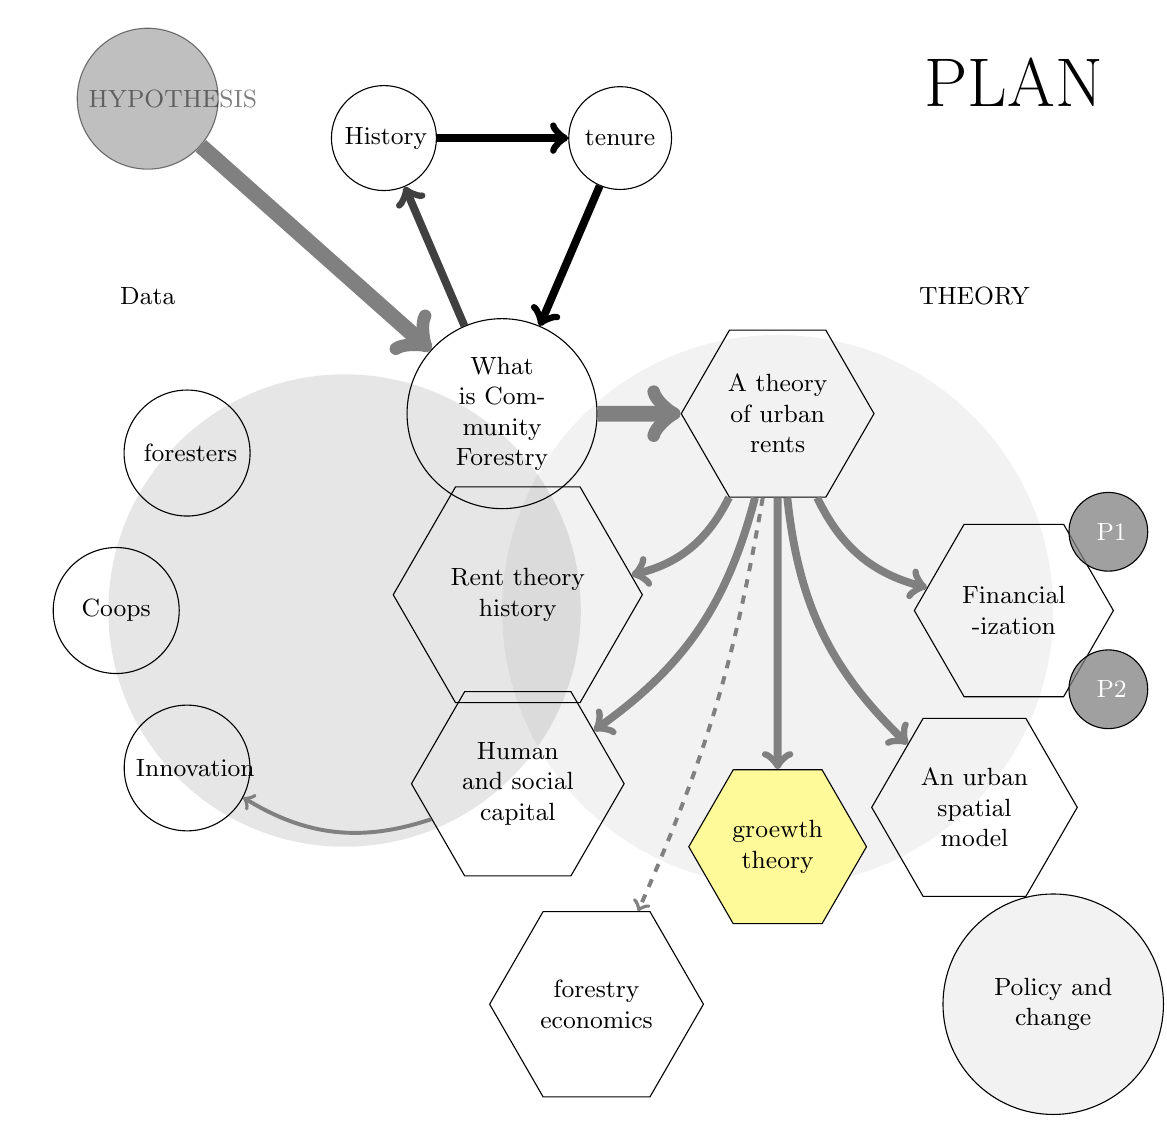
\begin{tikzpicture}%[scale=.8]
    \tikzstyle{every node}=[font=\small]
%\draw[help lines,step=.5] (0,-11) grid (11,11);

%  LOCATION OF ALL NODES
\coordinate (aa) at (-1.5,7.5);%PREFACE
\coordinate (a) at (-1,10);%
 \coordinate (b) at (1.5,7); %history
\coordinate (c) at (6,10); %
\coordinate (d) at (9,9);%
\coordinate (ee) at (-4,7);%
  \coordinate (e) at (-1.5,5); %Community label
\coordinate (f) at (9.5,7.7); %???    PLAN
\coordinate (g) at (9,5); %Economics label
\coordinate (h) at (4.5,7);%tenure
\coordinate (ii) at (-4,4);%
   \coordinate (i) at (1,4);  
\coordinate (j) at (3,3.5);%whatis
\coordinate (k) at (6,4);%
 \coordinate (l) at (6.5,3.5);%joint
\coordinate (mm) at (-1.9,1);%coops
 \coordinate (m) at (1,1);%community grey circle
  \coordinate (n) at (3,1); %
  \coordinate (o) at (9.5,1); %efficiency
				 \coordinate (oo) at (6.5,1);%
				  \coordinate (o1) at (10.7,2);	 \coordinate (o2) at (10.7,0);%Propositions
\coordinate (p) at (9,-1.5);%externalities
				
\coordinate (qq) at (-4,-2);
\coordinate (q) at (-1,-1);%innovation
 \coordinate (r) at (3.2,1.2);%trans
  \coordinate (s) at (3.2,-1.2);%capital
 \coordinate (t) at (6.5,-2);%pubgoods
\coordinate (AA) at (-2,-5);%
 \coordinate (A) at (1,-5);%
\coordinate (B) at (3.7,-4); %
\coordinate (C) at (4.2,-4);%forestryEC
\coordinate (D) at (-1,3);%foresters
\coordinate (EE) at (-1,-8); \coordinate (E) at (1,-8); \coordinate (F) at (3,-8); \coordinate (G) at (6,-8); \coordinate (H) at (10,-4);%Policy
\coordinate (II) at (-4,-11);  \coordinate (I) at (1,-11); \coordinate (J) at (3,-11); \coordinate (K) at (6,-11); \coordinate (L) at (10,-11);
%\coordinate (M) at (coordinate); \coordinate (N) at (coordinate); \coordinate (O) at (coordinate); \coordinate (P) at (coordinate);
%\coordinate (Q) at (coordinate); \coordinate (R) at (coordinate); \coordinate (S) at (coordinate); \coordinate (T) at (coordinate);

%.  CIRCLE NODES
% \fill[red, fill opacity=.8] (0,0) circle (4cm);
\fill [gray, fill opacity=0.2] (m) node [text width=2cm, black, opacity=1] 				(community)	{} circle (3cm);
\fill [gray, fill opacity=0.1] (oo)  node [text width=2cm, align=left, black, opacity=1] 		(econ) {} circle (3.5cm);
\node at (e) [ ] 		(comLtabel) {Data};
\node at (g) [ ] 		(ecLabel) {THEORY};
				%\draw (0,3.2,1) node [text width=1.5cm, text centered] {$Economics$};
			%\draw [fill=red, fill opacity=0.3]  (aa) node [ text width=2cm, black, opacity=1] 									(preface)		{PREFACE: Why, claims} circle (1.4cm);
\node [circle, draw,  fill=gray, opacity=.5,, text width=1.5cm] at			 (aa) 		(preface)		{HYPOTHESIS};
\node [] at			 (f) 		(plan)		{\Huge PLAN};
			%\draw [fill=blue, fill opacity=0.35] (b)node [text width=2cm, align=center, black, opacity=1] 			(history){History: New is Old} circle (1.2cm);
\node[circle, draw, text width=1cm, align=center, black, opacity=1]at 	(b)(history){History} ;
			%\draw [fill=pink, fill opacity=0.5] 		(h) node [text width=2cm, black, opacity=1] 								(tenure) 	{\color{black}tenure} circle (1.2cm);
\node[circle, draw,  text width=1cm, align=center, black] at 				(h) (tenure) 	{tenure} ;
\node[circle, draw,  text width=1.5cm, align=center]at							 (j) (whatis) 	{\color{black}What is Community Forestry} ;
\node[regular polygon, regular polygon sides=6, draw, align=center]at (l) (joint) 	{\color{black}A theory\\ of  urban\\ rents} ;


%\node[circle, draw,  text width=2cm, align=center]at (h) (tenure) 	{\color{black}tenure} ;

%\draw [fill=red, fill opacity=0.5] (j) node [text width=2cm, black, opacity=1] 												(whatis)		{What is Community Forestry}circle (1.4cm);
%\draw [fill=orange, fill opacity=0.5] 	(l) node [text width=2cm, black, text opacity=1] 	               		(joint)	{Joint products}											 circle (1.2cm);
%\draw [fill=green, fill opacity=0] (1,5)node [text width=2cm,red, opacity=1] {Policy and change} circle (1.4cm);
%\draw (q) node [text width=1.3cm, align=center, black, opacity=1] (small)	 {Innovation} circle (1.1cm);
\node[circle, draw,  text width=1.3cm, align=center] at							 (q) (small)	 {Innovation} ;

\draw 	(mm) node [text width=1.3cm, align=center, black, opacity=1] 	(coops) 	{Coops} circle (.8cm);
%\draw [fill=orange, fill opacity=0.5] 	(s) node [text width=2cm,  align=center, black, text opacity=1] (capital) {Human \\and social \\capital} circle (1.2cm);
\node[regular polygon, regular polygon sides=6, draw, align=center] at (s) (capital) {Human \\and social \\capital} ;
%\draw [fill=gray, fill opacity=0.5] 			(o) node [text width=2cm, black, text opacity=1] 						(efficiency)	{Efficiency} circle (1.2cm);
\node[regular polygon, regular polygon sides=6, draw, align=center] at (o) (efficiency)	{Financial\\-ization};
\draw [fill=gray, fill opacity=0.75] (o1) node [text width=.3cm, white, text opacity=1] (	P1)  {P1} 		circle (.5cm);
\draw [fill=gray, fill opacity=0.75] (o2) node [text width=.3cm, white, text opacity=1] (P2) {P2} 			circle (.5cm);

%\draw [fill=orange, fill opacity=0.5] (p) node [text width=2cm, black, opacity=1]					(externalities)	 {externalities} 			circle (1.2cm);
%\draw [fill=orange, fill opacity=0.5] (t)node [text width=2cm, align=center, black, opacity=1] (pubgoods) {public goods} 		circle (1.4cm);
%\draw [fill=orange, fill opacity=0.5] (r) node [text width=2cm, black, opacity=1] 							(trans)	{transaction costs} 		circle (1.1cm);

%.  POLYGON NODES
\node[regular polygon, regular polygon sides=6, draw, align=center] at (p) (externalities)	 {An urban \\spatial\\model};
\node[regular polygon, regular polygon sides=6, draw, align=center, fill=yellow!40] at (t) (pubgoods) {groewth\\theory} ;
\node[regular polygon, regular polygon sides=6, draw, align=center] at (r) (trans)	{Rent theory\\history};



%\draw [fill=yellow, fill opacity=0.15] 	(C) node [text width=2cm, black, opacity=1] 							(forestryEC){forestry \\ economics} circle (1.4cm);
\node[regular polygon, regular polygon sides=6, draw, align=center, fill=gray!.25] at (C) (forestryEC){forestry \\ economics};
\draw [] 	(D) node [text width=1.1cm, black, opacity=1] 							(foresters)	{foresters} circle (.8cm);

  %%%%%JOINT PRODUCTS  AND TRANSACTION COSTS
%\draw [fill=orange, fill opacity=0.5] (G) node [text width=2cm, black, opacity=1] 								{efficiency} circle (1.4cm);
  %%%%%%%%%%%%%%%%%%%%  POLICY CHANGE
\draw [fill=gray, fill opacity=0.1] 		(H)    node [text width=2cm, align=center, opacity=1] 										{Policy and change} circle (1.4cm);

% LINKS
%\draw (J) node [text width=6cm, text centered] {Economic Development };
%\draw ()--();
\draw [gray, line width=2mm,-> ](preface)--(whatis);
\draw  [darkgray, line width=1mm,<- ](history)--(whatis);
\draw  [black, line width=1mm,-> ](tenure)--(whatis);
\draw  [black, line width=1mm,-> ](history)--(tenure);

\draw [gray, line width=2mm,-> ](whatis)--(joint);
\draw [gray, line width=1mm,-> ](joint) to [bend right=25](efficiency);
\draw  [gray, line width=1mm,-> ] (joint) to [bend left=20](capital);
\draw [gray, line width=1mm,-> ](joint) to [bend right=20](externalities);
\draw [gray, line width=1mm,-> ](joint) to [bend left=25](trans);
\draw  [gray, line width=1mm,-> ](joint)->(pubgoods);
\draw  [gray, line width=.5mm,-> ](capital) to[bend left=25](small);
\draw  [gray, line width=.5mm,-> ,dashed](joint) to[bend left=7](forestryEC);
\end{tikzpicture} 

\end{document}
%     \caption{Caption}
%     \label{fig:my_label}
% \end{figure}


\chapter{Resilience analysis}
% - 0. basic hysteresis/irreversibly result 1. Pumps wealth out on way up and way down 2. class 3. map regimes


\begin{figure}
\centering
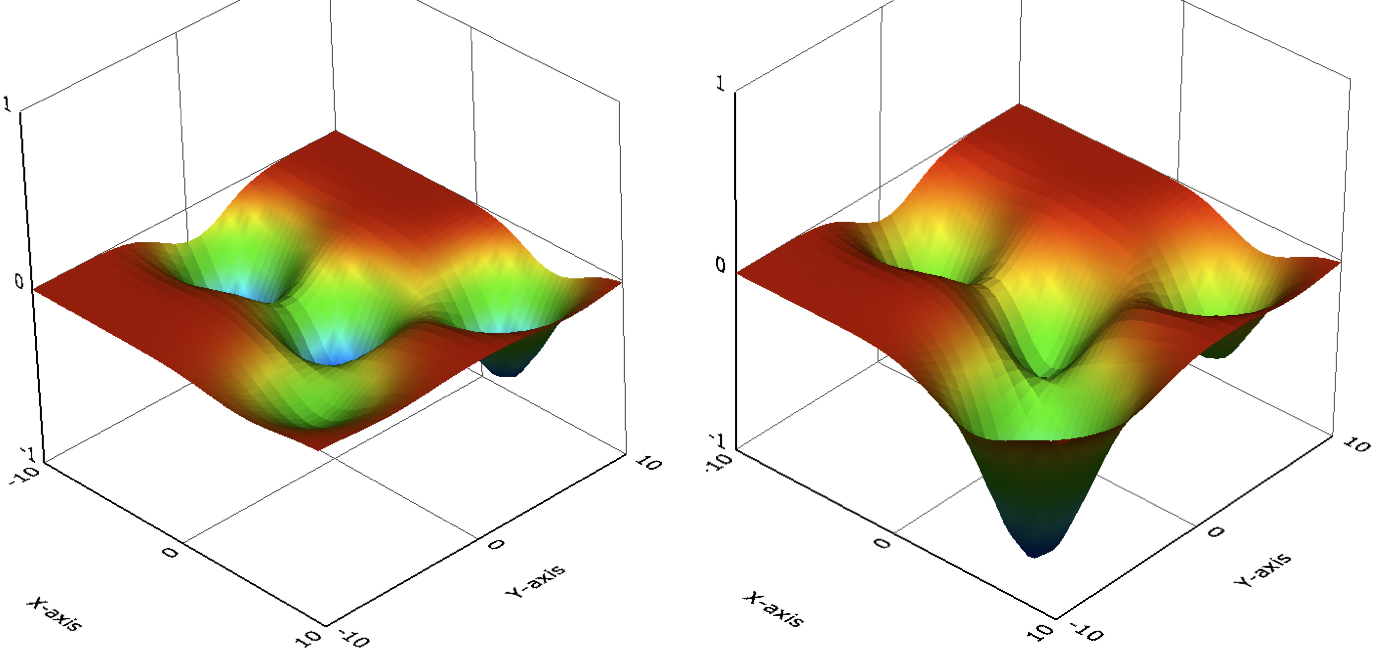
\includegraphics{fig/basins.png}
\caption{Basins of attraction}
\label{fig-basins}
\end{figure}

Historically low interest rates, and financial crises, have been a primary driver of rapid inflows of financial capital, accelerating the process, which raises the question of what will happen as interest rates rise. The analysis suggests however that there is hysteresis, that both the economic upswing and the downswing pull wealth out of communities, like a kind of ratchet or peristaltic pump. We analyze and model these dynamics in the resilience Chapter, %Chapter~\ref{chapter-resilience}

The model gives a resilience result which is that shared wealth through housing is not resilience.

It can also be used with a driven version of the model to show that the model pumps wealth out on the upswing and on the downswing - like a kind if ratchet.


Once we have this model it is useful for also understanding the wealth effects, in particular the resilience dynamics
Resilience is an under used concept in economic analysis for a few reasons. We show an example of that type of analysis based on hysteresis here. 


There are two types of resilience questions when any system is shocked, does it return to an equilibrium state, the stability question, and does it return to the same kind of equilibrium---the hysteresis question. % We focus on the latter question.  

\section{Definitions of resilience}

The concept of resilience has been used to understand the persistence and vulerabilty of high dimensioanl social and ecological systems %\cite{several reviews}
but is usually defined either verbally or formally in terms of low dimensional dynamical systems. Recent work has begun to look at how to extend it to higher dimensional systems \cite{gao_universal_2016}. 

Litturature on resilience is part of a larger body of work on several distinct stability concepts. 
Grimm and Wissel reviewed stability terms from the ecological literature \cite{grimm_what_2011, grimm_babel_1997} and identified three core underlying concepts \footnote{They reviewed 163 definitions and 70 distinct terms.}. The first was \textbf{constancy}, the degree to which the some element of a system resists perturbation. The second was engineering resilience, the ability of a system to \textbf{bounce back} from a disturbance.  The third was the \textbf{viability of some feature of a system in the long term}. % Did the property actually die out or did it last?

The concept of resilience from the ecological literature is related to this this final stability concept. Holling originally defined resilience as determining ``the \textbf{persistence of relationships within a system}.'' It is, he continues, ``a measure of the ability of these systems to absorb changes of state variables, driving variables, and parameters, and still persist” \cite{holling_resilience_1973}. %(Holling 1973, p. 17 - checked page and quote DONE) %In this definition resilience is the property of the system and persistence or probability of extinction is the result.


% Ludwig, Jones and Holling, Qualitative analysis of insect out- break systems: the spruce budworm and forest , Journal of Ani- mal Ecology (1978), 47 , 315-332.2. Polking, Boggess and Arnold, Differential Equations , 158-161. October 6, 1977 issue of Nature Magazine (Vol. 269, pg. 471)

His definition was developed in the context of this formal modelling but was itself verbal and qualitative. More recently Walker et al. define resilience as %``Resilience is 
``the \textbf{capacity of a system to absorb disturbance and reorganize while undergoing change so as to still retain essentially the same function, structure, identity, and feedbacks}'' \cite{walker_resilience_2004}.
 % Resilience is the capacity of systems to maintain their identity, feedbacks, structure, and pattern of functioning as they pass through transformations. 
Empirically, Marten Scheffer and others look at %who developed a toolkit for measuring advance indicators of critical transitions, define 
measure resilience using the ``\textbf{magnitude of disturbance a system can tolerate before it shifts into a different state}'' \cite{scheffer_critical_2009}.
% (Critical Transitions in Nature and Society, Dakos critical transitions advance warning toolkit website glossary has this as the definition of resilience)



Work on networks and resilience defines resilience as ``a system’s \textbf{ability to adjust its activity to retain its basic functionality} when errors, failures and environmental changes occur'' \cite{gao_universal_2016}. %(Gao et al. 2016). 
They say this has traditionally been defined for ``low-dimensional models with a few interacting components'' in the following way:
% For the low dimensional defintion, they cite Sole, R. V. & Montoya, M. Complexity and fragility in ecological networks. Proc. R. Soc. Lond. B 268, 2039–2045 (2001) ** 

\begin{equation}
   \frac{dx}{dt} = f(\beta, x)
\end{equation}
Where $f(\beta, x)$ is the system's dynamics, $\beta$ is changing environmental conditions, and the system has several stable fixed points or regimes. The system begins near at one of the fixed points and is initially stable.

\begin{equation}
   f(\beta, x_0) = 0
\end{equation}

\begin{equation}
   \frac{\partial f}{\partial x} \bigg|_{x = x_0} < 0
\end{equation}
Over changes in the tunable parameter $\beta$, the system can reach a biffurcaiton or become non-analytic, and transition to an alternative stable state or regime.

Neubert and Caswell describe a range of measures for how ecological systems respond to perturbations \cite{neubert_alternatives_1997}. These include the
rate at which perturbations decay, % to stable equilibrium decay, most often based on the eigenvalues at equilibrium, which gives rate of recovery asymtotically as time goes to infinity, and % (copied note. check this is paraprhased properly) %New measures of transient response
reactivity, and the maximum possible growth rate immediately after perturbation.
%'These indices measure the extent and duration of transient growth in models with asymptotically stable equilibria. They are: 

%\begin{enumerate}
%   \item \textbf{reactivity} (the maximum possible growth rate immediately following the perturbation), the 
%   \item \textbf{maximum amplification} (the largest proportional deviation that can be produced by any perturbation), and the 
%   \item \textbf{time at which this amplification occurs}. 
%\end{enumerate}


%------------------------------------------------------------------


% [1] J. Gao, B. Barzel, and A.-L. Barab ́asi, “Universal resilience patterns in complex net- works,” Nature, vol. 530, no. 7590, pp. 307–312, 2016.
% [2] V. Grimm and J. M. Calabrese, “What is resilience? A short introduction,” in Viability and Resilience of Complex Systems, ser. Understanding Complex Systems, G. Deffuant and N. Gilbert, Eds. Berlin: Springer, 2011, pp. 3–13.
% [3] V. Grimm and C. Wissel, “Babel, or the ecological stability discussions: An inventory and analysis of terminology and a guide for avoiding confusion,” Oecologia, vol. 109, no. 3, pp. 323–334, 1997.
% [4] C. Holling, “Resilience and stability of ecological systems,” Annual Review of Ecology and Systematics, vol. 4, pp. 1–23, 1973.
% [5] B. Walker, C. S. Holling, S. Carpenter, and A. Kinzig, “Resilience, adaptability and transformability in social-ecological systems,” Ecology and Society, vol. 9, no. 2, 2004.
% [6] M. Scheffer, Critical Transitions in Nature and Society, Princeton, 2009.
% [7] M. G. Neubert and H. Caswell, “Alternatives to resilience for measuring the responses
% of ecological systems to perturbations,” Ecology, vol. 78, no. 3, pp. 653–665, 1997.

\subsection{Endogenous cycling}
Paul suggests that resilience is usually studied in the context of a system which endogenously shifts between two alternative regimes.

This is false, in the vast majority of cases resilience in ecological systems is studied in the context of a system which 

That being said, endogenous cycling is caused by a feedback cycle which causes the system to cycle between distinct high and low employment regime within a single region of the state space.

There is also a region near the boundaries, kicks to state through endogenous randomness can also cause the system to cross the boundary from one region to another.


\section{Resilience background}

This section explores the resilience dynamics of distribution of wealth within a class of market models.  

Using a systems design approach and looking at resilience measures and alternative regimes gives insights into patterns of distribution and how that shapes wealth. 

The two significant concepts of resilience for this work are the relationship between distinct alternative regimes and patterns of cycling within a single regime. 

\section{What is resilience and how is it connected to this work}

Resilience is a concept that has to with the way in which a system resists disturbance or maintains identity through disturbance. The concept has emerged independently with different, but related definitions in various fields. 
There are a class of systems that this idea of resilience should be applicable or illuminating for, however the concepts and measures that exist already are ill-suited to the dynamics of the system. 
The work in this thesis draws from the measures from existing measures and concepts of resilience from various discipline to evolve a measure that can apply to this other class of systems. 

Shaping this core broadly applicable concept that 
We can approach change in various systems using technical tools that are transferable. 
The concept 

\section{Resilience in engineering}

In engineering, Resilience is defined as the return properties of a system. 
It is the measures relating to how a system comes back to its stable equilibrium or stable state. For example if you push a branch on a tree, it will oscillate and settle back to its resting position. 

Stability properties are important in engineering because engineers are responsible for signing off the performance of system, whether the the system is a bridge or a chemical reactant or an electrical circuit. Stability is an aspect of the system's behaviour. The engineer needs measures to predict the stability of the system when it's perturbed. (Specific) 

Engineering resilience is distinct from the failure zones or the threshold of failure - for example the level of force/weight or number of stress cycles that would be required to collapse a bridge. While those measures pertain the thresholds beyond which the system would fail, resilience is about describing how the system recovers from perturbations that do not break it. 

The primary measure is how long the system takes to return to its equilibrium, i.e. the return time. (Equation) There are seven measures, listed in table XYZ that pertain to return to equilibrium properties.  (Table)

There is some variation in the use of the concept in specific disciplines of Engineering. For example, in transport engineering it has something to do with traffic flow.

\section{Resilience in ecology}

In Ecology resilience is defined as the way in which systems maintain identity through transformations. 

In engineering, the concept of resilience centres on the idea of a single equilibrium. If the system is not disturbed, it will stay at equilibrium and the resilience measures account for the system's return to this equilibrium. In the ecology, on the other hand, instead of a single equilibrium the underlying pattern of the system has a dynamic structure. For example the ecosystem of a forest contains ongoing cycles of life and death and evolving patterns and interactions and yet sustains its identity as a forest. 

An ecosystem can experience big shocks or disturbances without losing its basic identity. For example, there can be drought, floods, fire, species loss, etc and the forest can recover and continue to be a forest. (The forest can regrow, one species might replace another and the forest changes but it doesn't necessarily stop being a forest.) But some disturbances can tip the ecosystem over into a different pattern of functioning. For example if the land is cleared and animals come into to graze the seedling trees so that they do not grow back, the forest can transition to a grassland ecosystem. Or if the region becomes dry enough, the forest can transition to become a desert. 

In ecology these alternative patterns of a system that may be identified as a forest, grassland, or desert are called regimes. In Ecological resilience studies, this concept of regimes replaces the simpler idea of equilibrium, differing both because the underlying pattern is more complex and because there are multiple regimes that the ecosystem of the same land can shift between. 

Part of what resilience in ecology is getting at, then, is what kind and how big the disruption can be before the ecosystem becomes a different kind of ecosystem. Resilience measures describe the properties of these distinct regimes and the relations between them. The most common measure is the size of the perturbation the system can withstand without transitioning into an alternative pattern of functioning or regime.  

This approach to resilience was introduced by C.S. Holling with his 1973 paper on a Spruce Budworm model of a forest ecosystem. In this paper he argued that there was an evolving interrelationship/feedback cycle between Spruce growth/regrowth and the population of Spruce Budworms that eat them. This interaction drove ongoing cycles of forest recovery and collapse. 

Holling's work established the concept of these kinds of cycled and alternative regimes in ecosystems. Subsequent work by Marten Scheffer in lake eutrophication validated that alternative regimes appear in ecosystems in the real world. Now there is a database tracking thresholds and regime shifts in ecological systems with over a hundred entries showing its common.  ([https://www.resalliance.org/thresholds-db](https://www.resalliance.org/thresholds-db)) 

In ecology, this idea of resilience has evolved into a dynamic concept that is important in climate change science and ecological conservation. Resilience measures show how a system maintains identity through change by measuring the relationship between regimes, that is how close a system is to transitioning to a different regime or pattern of functioning. Thus the concept of ecological resilience and alternate regimes give tools to understand what is possible for an ecosystem. This give insight both into how ecosystems can be preserved but also what happens when they transform. 




\section{Resilience in social systems}

The ecological concept of Resilience has since been applied widely to various systems across disciplines (*INSERT EXAMPLES*). Frances Westley applies Holling's idea of alternative regimes to social systems as the basis for a theory of social innovation. 

Westley defines social innovation as ``a change in the routines, resource flows, authority flows or beliefs in any social system.'' According to Westley ``a successful social innovation also has durability and broad impact.'' 
Her studies in social innovation focus on how individuals, groups, or institutions are able to shift social systems to achieve certain goals. 

Westley's research question is how social systems transform. This frame differs from the majority of resilience work in engineering and ecology because the focus there tends to be on maintaining the integrity of the system, whereas Westley's work is focused on how to move between regimes. 

For example, in the Great Bear Rainforest in British Columbia in the late 1990's (??) clearcutting for pulp and paper was threatening some of the last old old growth forests in the region and disrupting the lives of people who depended on them. Over years of unchecked logging combined with a history of land appropriation, there was ongoing local resistance. In 199X images of the devastation spread through international media and led to a boycott of paper products from clearcutting. This moment of crisis brought the forestry industry to the table. After a carefully structured process of conversation and engagement between community organizers, political leaders, and industry they put the Great Bear Rainforest under Indigenous community control. 

This change in governance structure can be understood social system that can be understood as a regime change because there were a set of patterns and feedbacks holding the old system in place and and there new set of patterns and feedbacks holding the new system in place. Each regime has a distinct pattern of functioning or identity. 

The idea of resilience in social innovation illuminates how the patterns of different regimes structure the social systems. What is different about the two regime in the case of the Great Bear Rainforest is the distribution of the flow of money and power - or the the language of social innovation, resources and authority. This changed the routines and habits of the people making up the social system as they became more directly involved in managing the forest. The result is that the ancient Great Bear Rainforest survived. 

The study of resilience within social innovation looks at how actors within  systems play a role in shaping transformation of interconnected social-ecological systems. Westley specifically studies individuals, groups, or institutions who have the intention to shift social systems to achieve certain goals. This means that there is a directed strategic nature to the agents. This is illustrated by the case of the Great Bear Rainforest by the different stakeholders from industry, community and governance who are are all actively working to achieve specific goals. However none of these actors are outside outside the system. Even those with power cannot completely control the system. Their efforts interact with the actions of others and the broader context of the whole

Social systems are dynamic. There is no fixed equilibrium and yet they have clusters of properties that persist and can prove difficult to change. These patterns with distinct identities are described in social innovation theory as regimes. These patterns can pertain to various feature, from the routines that structure interactions to resource flows within the system. In the example of the Great Bear Rainforest, under the previous system the resources and money flowed out of the community and decisions were made by distant corporations. The shift in governance structurally affected both the ecosystem and the culture of the communities. When they shifted to community governance, the emphasis shifted away from extraction and toward investing and building the forest and the community. (ADD CONCRETE DETAILS/NUMBERS?) 

Sometimes people can achieve their goals and sometimes they do not and it depend on both what they do and the state of the system. In her grounded theory work studying people who have attempted and succeeded in changing systems, Westley observed that sometimes there are moments of opportunity that make shifts in the system possible.  In the rainforest example, there were years of Indigenous organizing and building an environmental movement. 
The change became possible at a particular moment when commodity prices were placing pressure on the industry and coordination between local and national environmentalists resulting in international boycotts of pulp and paper products from clearcut forest, particularly across Europe. The indigenous organizers were able to achieve more in this moment of opportunity.

According to Westley a successful social innovation also ``has durability and broad impact.'' This is a description of the change but it also illuminates how the resilience concept of regimes is useful. One feature of systems is that a set of feedback loops will hold patterns of interactions, resources flows, etc in place. Many changes simply die out.  The changes that last do so because they change the flows and dynamics in ways that are held in place by new feedback loops.  Social Innovation theorists have used the concept of regimes to explain this phenomena. If the system state is perturbed enough another set of patterns can come to dominate.  (MAKE SURE THESE TERMS ALIGN WITH THE PRECISE TERMINOLOGY USED LATER) In the example, after the shift to the community governance that became self-reinforcing as different feedback loops emerged to structure the building of relationships and institutional structures, community habits, networks of support, and resource flows. 

\section{Role of this thesis}

What has been articulated in Social innovation theory is a story of how feedback loops hold the patterns in place  and how systems can switch between sets of patterns. Westley and others have applied the concept of resilience as an explanatory framework, rather than as a a precise mathematical statement. 
The thesis seeks to operationalize these concepts within a formal model in the context of social systems. 


- By operationalizing into this model, we can patterns in how systems shift between regimes. Specifically in this thesis the models show where in the systems there are opportunities - ie the system is more vulnerable or -open to change. 
- In practice regimes change can move you into a more or less desired state. Here I focus on opportunities and interventions. 
- Inventions are \dots
- By looking at where the system has opportunity to change this work illuminates how actors might be able to identify opportunities for regime change. 
- 




prosperity and resilience/vulnerability/opportunity in the context of many agents.











he analysis has been applied conceptually, rather than as a precise mathematical statement. Thus far, in the study of social innovation 

Routines, resource authority flow and beliefs. 

International concern
Boycotts 
Political movement

Effective local movement established an indigenously led sustainable forest and tenure
It 



Community leaders were able to establish a 




Social innovation involves interventions or actions 




She studies I

Change in technology and demand for wood. 

For example, she looks at how various countries responded to the AIDS crisis and how activists in certain shaped 

There's a debate about how systems transform. 
Impersonal forces of history like the development of agriculture
She's studying the phenomena of change in order to inform 
The research is about how people try to change the word. 

(ie. a system consisting of different interconnected entities such as  individuals, groups, and institutions relating to each other and forming a whole.)

An interdependence of a social and cultural element 

Series of interrelationships between individuals and groups and institutions forming a whole. 



% [[adaptive cycle]]




Recreate their images in low resolution (\textbf{phase diagram, example trajectories, policy performance}).

Alternative experiment ideas include:

\begin{enumerate}
\item Find and trace the boundary by brute force. They currently use mean field approximations or \textbf{brute force simulations} to identify the phases, barriers and regimes/patterns in phase diagrams of the economy (add detail).
\item Find and trace the boundary by ab initio methods. Try ab initio methods from chemistry to find and \textbf{trace the boundary}. Identify a generic regime boundary. Identify latent alternative states.
   \item \textbf{Characterize the boundary}. Characterize save/dangers near regime boundaries.
   \item Systematically \textbf{vary the model} in the direction likely to change the set of patterns of behaviours. \textbf{Identify new phases}, patterns without knowing them in advance../new regimes.
   \item Systematically explore/intelligently explore a space of alternative \textbf{interventions}.. — select hyper-parameters/model the parameter space. Model/think about the geometry of the intervention space/and the dimension of it.. — ways to control what levers.. in time, space, etc..? VERY LARGE SEARCH SPACE ETC..
   \item Characterize/link with the \textbf{adaptive cycle} — connectivity wealth, etc..
Adaptive cycle currently treated as metaphorical .. measure the predicted effect in these models and compare with data.. capital etc..
\item Look at \textbf{traps}, and interventions using an energy \textbf{barrier framework}.
Phenomena including the \textbf{Paradox of thrift, Liquidity traps.}
\item \textbf{Network efficiency} and others under different classes of attacks? measure of economic efficiency with frictions, capital, trust etc.. recovery times. e.g. Trust collapse network sizes.
\item \textbf{Math of paradigm shift in stylized model} - openings through cycling. resilience and the adaptive cycle — a cycle that allows for adaptation.. FILL IN DETAILS.


\item Look at the effect of money on the shape of endogenous crises
\item Look at the effect of advance/pre triggering of endogenous crises
\item Look at methods to reduce/change the depth of crises/peaks
\item Compare one large intervention with continuous intervention and lots of small interventions, look at timing effects.

\item The high-throughput highway to computational materials allows comparison of a whole class of models and policy inventions..

\item The way to study this is to study 1. model changes 2. policy changes (geometry of the system). 
\end{enumerate}





\section{How to compare multiple replicate runs?}

Compare with standard deviation (CV is a dimensionless form of this)

You could look at the\textbf{ Standard deviation} (SD) or \textbf{Standard Error of the Mean} (SEM) which will give you an idea of how close the replicate values are to each other.  


``The standard error of the mean (SE of the mean) \textbf{estimates the variability between sample means that you would obtain if you took multiple samples} from the same population. The standard error of the mean estimates the variability between samples whereas the standard deviation measures the variability within a single sample.''

best way to calculate the variability between assays and duplicates/triplicates is \textbf{CV=(SD/mean)*100}. The lower CV the better, It should be less than 20\%. 
I think some people use <15 percent CV as a valid result, if it is higher than 15\%, then you shouldn't consider that duplicate/triplicate.

``In order to express the precision, or repeatability, of immunoassay test results, rresearchers in the social and  behavioral sciences typically report two measures of the \textbf{Coefficient of Variability}  (CV) in their publications:  the  Inter - Assay CV and the Intra - Assay CV.  The CV is a dimensionless number defined as the \textbf{standard deviation of a  set of measurements divided by the mean of the set}. ``

`` The degree to which the duplicate results differ 
can be expressed by calculating t
he standard deviation of the two results and converting it to the CV. ``
\cite{https://www.salimetrics.com/assets/documents/Spit_Tips_-_Inter__Intra_Assay_Coefficients_of_Variability.pdf}


``If \textbf{absolute values are similar, populations can be compared using their standard deviations}. But if they differ markedly (for example, the weights of mice and elephants), or are of different variables (for example, weight and height), then you need to use a standardized measure - such as the coefficient of variation. The coefficient of variation (CV) for a sample is the standard deviation of the observations divided by the mean. The most common use of the coefficient of variation is to assess the precision of a technique. It is also used ass a measure of variability when the standard deviation is proportional to the mean, and as a means to compare variability of measurements made in different units.''
\cite {https://www.researchgate.net/post/How_to_calculate_the_inter_assay_and_intra_assay_vatiations }



\subsection{What are replicat runs vs repeats}
(assume the system is stationary?)

'Replicates are multiple experimental runs with the same factor settings.' 'Repeat and replicate measurements are both multiple response measurements taken at the same combination of factor settings; but repeat measurements are taken during the same experimental run or consecutive runs, while replicate measurements are taken during identical but different experimental runs, which are often randomized.'
\cite{http://support.minitab.com/en-us/minitab/17/topic-library/modeling-statistics/doe/basics/replicates-and-repeats-in-designed-experiments/}
``Replicates are duplicate runs of the entire experiment.
The latter is preferable for minimising errors. Sample size calculations apply to replicates not repeats.''

I need to actually calculate the CV for each sample: \cite{http://r.789695.n4.nabble.com/Need-to-calculate-within-and-between-run-CV-td866024.html}
  - within run (between replicates) - that's easy to do in Excel
  - between run - that's the problem.
  aov' or 'lme'? 

\chapter{Resilience and class}

(TODO: introduce the idea of class in the resilience section, and link it to the resilience of the wealth trajectories.)  
reversibility/hysteresis, and how class is treated in the literature.
Three spatially segregated `classes.' Capitalists live in some spaceless utopia,  Urban workers who commute and earn wages in the urban commuter-shed, and  rural residents and landowners who may choose to move to the city. There may be a band surrounding the city or persons who do not commute but enjoy urban consumption amenities. 
a fourth class, the urban tenant. 
Developed in Chapter~\ref{chapter-model} on modelling.

The model is we employ consistent with the theories of Ricardo and Henry George in locating the ground of urban exploitation and class in the capacity to extract social surplus through land ownership, and differs from the standard Marxian analysis in its reliance on access to financial capital rather than control of productive physical capital. The paper concludes that given existing land ownership patterns which encourage speculative investment, housing prices must rise and income inequality must increase. 

In the classical language, someone is exploited if someone else gets a share of the value of their labour. %(REPLACE WITH MORE PRECISE DESCRIPTION). 
 Employers capture a share of the value of workers' labour, so they exploit workers under this definition.
Those who own land early in a growing city are also capture a share of everybody's production. Since they capture a share of the productivity of others working in the city, through the rents, they are also exploiters, they form a kind of hybrid class. %Rents could be captured directly through renting out the property after they retire away from the city,  or by selling the property at a higher value than they bought it. 




\section{Class}
We use the concept of \gls{class} to explore the consequences of financialization in the housing market. The term class was used  by classical and Marxist economists to refer to patterns in the ownership of productive assets.\footnote{ Erik Olin Wright summarizes the approach common to classical and Marxist analysts:  ``The fundamental contrast in capitalist societies, for example, is between owners of means of production and owners of labor power, since `owning' is a description of rights and powers with respect to a resource deployed in `production'\thinspace'' \cite{wrightAlternativeFoundationsClass2002}.} Those who had only their labour to sell were \gls{working class}. Those who lived off the rents from the land they owned were \glspl{landowner}. Those who captured the surplus from industrial production because they owned the capital stock were capitalists, and those who lived off the the income from property or money lent were \glspl{rentier}.\footnote{The term rentier is used variously. It is applied to people living off the income from already acquired wealth, and applies, for example to pensioners.  In `rentier capitalism' it is a noun meaning: a business model in which ownership of key types of scarce assets-such as land, intellectual property, natural resources, or digital platforms-is all-important and dominated by a few unfathomably wealthy companies and individuals called rentiers.} 

\begin{table}[!ht]
    \begin{centering}
\begin{tabular}{lcccccc}\small
  
    & \multicolumn{6}{c}{Means of Production}\\   \cline{2-7}
     &labour &talent & education& land & \multicolumn{2}{c}{capital} \\ \cline{6-7}
     &       &       &          &       &real   &financial  \\ 
     \hline
      \multicolumn{7}{c}{working classes}\\
simple& X   &       &         &         &       &\\
gifted& X   &    X  &         &         &       &\\
professional& X   &       &    X   &         &       &\\\hline
& \multicolumn{6}{c}{middle classes}\\  
   \multicolumn{7}{c}{lower}\\
Middle  & X   & * & X  & +&  + & +\\
classes & X   & X & *  & + & + & +\\\hline

 & \multicolumn{6}{c}{upper (\textit{working owners})}\\
% \multicolumn{7}{c}{}\\
landowner & X  &   *   & * &   X   &   *  & * \\
capitalist& X  &   *   & * &   *   &   X &  *\\
rentier   & X  &   *   & * &   *   &   * & X\\\hline

&&&& \multicolumn{3}{c}{pure owners}\\
landowner  &   &  & &   X  &       &\\
capitalist &   &  &  &     & X  &\\
rentier    &   &  &  &     &   & X\\ \hline
\end{tabular}
\end{centering}
\vspace{.25cm}

``\textbf{X}'' and ``\textbf{+}'' together indicate class identification

``\textbf{+}'' signs in a given row indicates `` at least one of these is included.''

\noindent``\textbf{ * }'' signs in a given row indicates `` may be included.''
\caption{Classes by asset ownership}
\label{table-classes}
\end{table}
% \usepackage{xcolor}
% \usepackage{nicematrix}
% \begin{document}
% \begin{NiceTabular}{lllllll}
% \CodeBefore
%   \rectanglecolor{blue!20}{2-2}{6-6}
%   \cellcolor{green!20}{7-7}
% \Body
%   & 1 & 2 & 3 & 4 & 5 & 6\\
% 1 & 1 & 1 & 1 & 1 & 1 & 0\\
% 
% 6 & 0 & 0 & 0 & 0 & 0 & 1\\
% \end{NiceTabular}
% \end{document}


This basic classification is too simple, of course. To describe a real society more fully, it has to be completed with a variety of sub-classes and intermediate classes. Table~\ref{table-classes} illustrates one approach based on Roemer's  \textit{A general theory of exploitation and class} \cite{roemerGeneralTheoryExploitation1982}. Variations in assets generate distinct professions, identities and alliances far more complex than a simpler version would suggest. The model allows for mobility between classes of the sort we suggest is occurring as a result of financialization of the housing market.

Workers, for example, who sell not just their labour, but also their talents and/or the services of their education will earn more as a rule and live better. Talents may include native skill in carpentry or coding, or beauty. Education includes the long apprenticeship of talented artists and  trades training as well as postsecondary education, management experience, or experience on wall street. It is worth noting that education is achieved by investment and is a capital asset, while talent is a gift of nature like land. 

The middle classes are especially complex because of the variety of assets individuals may own. The traditional shop owner, for example, often described as a member of the \gls{petite bourgeoisie}, may work in his own a shop and with his equipment and enjoy a relatively comfortable income, but still  need to apply his own labour. The professional classes have skills as a result of their investments in learning their profession. the market value of their human capital may be increased by professional organizations that restrict entry to the profession, and augmented by social capital.  Despite the similarity between the craft trades and the professional trades, the latter generally have greater social status. Consideration of social  further complicates discussions of class.

One of our goals is  to show how financialization of the housing market drives change in the class mix within cities using this asset-based understanding of class.





we could also think of location as among them





\section{Investment amplifies the problem of financialization}
If the problem is not a supply problem, investment makes it worse and increases vulnerabilty.

\subsection{financialization amplifies the problem of housing shortages }

\begin{enumerate}
    \item to model set a low alternative $i$ and then put a dial on the amount of K in any period (this is friction)
    \item Vary individual costs of capital - the function that raises the rate for the poorer buyers can be made steeper.
    \item How do we make $\dot p$ more volatile - this feeds into developer decisions
\end{enumerate}

This will accelerate tenantization.

\subsubsection{holding property for later development}

\begin{enumerate}
    \item We need a density function. Redevelopment is increasing density. Unit size (land per unit) is constrained by a utility function  (but only for newcomers, I think.) 
    \item with a density choice increasing density can be delayed.
    \item you could even set a hard boundary on the city and just explore density. 
    \item We need a way to increase population pressure. (maybe just amplify the wage
\end{enumerate}
If it's not a supply problem
Leaning into rental removes a key piece of how we've build the model


Would get pieces held off the model.
get units held off the market.


Model to hold the developer.. 
Need a density function, go to a different density..
look to see when it's better to wait to invest in increasing density.

\subsection{Class structure} \label{section-class-structure}
At the stage illustrated on the right  in Figure~\ref{fig-rent-driving},  %(Alonso city suburbanized with owner occupiers) 
as a result of rapidly rising productivity, falling transportation costs, and large amounts of land with relatively low productivity, a new urban social system has emerged with a land-owning working class. 

The term \gls{class} is often used informally as if it refers straightforwardly to people who have different levels of wealth, but when economists talk about classes, they usually mean something slightly different. Economic classes are functionally defined:  by how they participate in production. Owners of labour participate by supplying their labour, for which they are paid a wage. Landowners own the land and receive rents for the use of their land in production. Owners of capital provide funds for starting and operating businesses, for which they receive profits.  There are three classes in this model and three kinds of income.  %It's because the surplus is differently distributed that different have different wealth levels. 

This emergence of a land owning working class is a recent phenomenon, and perhaps primarily a North American one. We are concerned in this thesis with whether may also be a passing stage.

America's economic transformation in the early 1800s was linked to dramatic changes in transportation networks. The construction of roads, canals, and railroads led to the expansion of markets, facilitated the movement of peoples, and altered the physical landscape. The later commuter transportation revolution further transformed cities and class structures.

It is partly a product of housing and transportation.
LINK BACK TO THE TRAS

Class, hysteresis, irreversibly.

\section{Extensions of the Alonso model}

The Alonzo model has been used to illustrate a wide range of urban issues. Incorporating these extensions, we can explore relatively fine-grained effects of financialization. The examples that follow  illustrate   ways the model can be applied and suggest further hypotheses that we  would like to test using our model.


\subsection{Differential transportation costs}
 Urbanists agree that before the railroad and the automobile, the extent of a city was roughly determined by how far a person could walk in about an hour. The time and effort cost of transportation determined the size of cities. 
 
 It also affected the distribution of the classes within the city. When everyone walked, the  wealthy may have valued their time more than the poor. In terms of the model, the willingness to pay of the rich would higher  near the core than  the willingness (or ability) to pay of  the poor, but would descend more rapidly with distance
\begin{figure}
\begin{center}
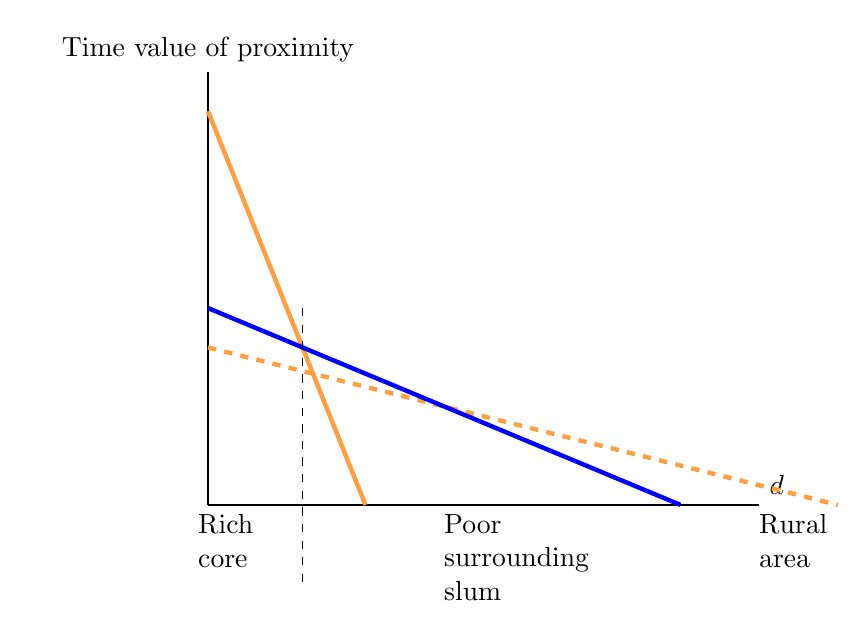
\begin{tikzpicture}[scale=1]

\draw[thick](0,0)--(0,5.5)node[above]{Time  value of proximity}; %Y
\draw[thick](0,0)--(7,0)node[above right]{$d$}; %X

\draw[ultra thick, orange!75](0,5)--(2,0);
\draw[ultra thick, orange!75, dashed ](0,2)--(8,0);
\draw[ultra thick, blue](0,2.5)--(6,0);
% \node[draw=white, fill=white] (b) at (1,2.9) {Rich};
% \node[draw=white, fill=white] (b) at (3,1.25) {Poor};
\draw[dashed](1.2,2.5)--(1.2,-1) ;
\node[text width =1cm, below left] at (1,0){Rich core};
\node[below, text width =2cm] at (4,0){Poor \\ surrounding slum};
\node[below, text width =1cm] at (7.5,0){Rural area};
% \draw[ blue, dashed](0,5)--(15,2.5);
% \node[circle,draw=black, fill=white, inner sep=3pt,minimum size=10pt] (b) at (7,3.75) {3};

% \draw[ blue, dotted](0,6.75)--(15,4.25);
% \node[circle,draw=black, dotted,fill=white, inner sep=3pt,minimum size=10pt] (b) at (7,5.5) {4};
\end{tikzpicture}\end{center}
\caption{Differing transportation time cost and housing distributions.}
% \label{fig_fix_my_label}
\end{figure}

 If the technology suddenly provides the rich with commuter trains or automobiles and more attractive sites at the edge of the city, the orange line could drop enough  and become much flatter leading in a flight of the rich to the suburbs, as appears to have happened in many American cities. Lower transportation costs make cheaper land on the edge of the city attractive. This would  offer  more space and the opportunity to build larger homes, a pattern that has emerged in some cities.



\subsection {Changing transportation costs}

Another application of the model is to the effect of a transportation revolution. The advent of first rail transportation and then the automobile radically changed the size, productivity, and population distribution of cities.
periphery available, allowing larger lot sizes and larger homes for those who can afford them.

\begin{figure}
\centering
% CHANGING TRANSPORTATION COSTS
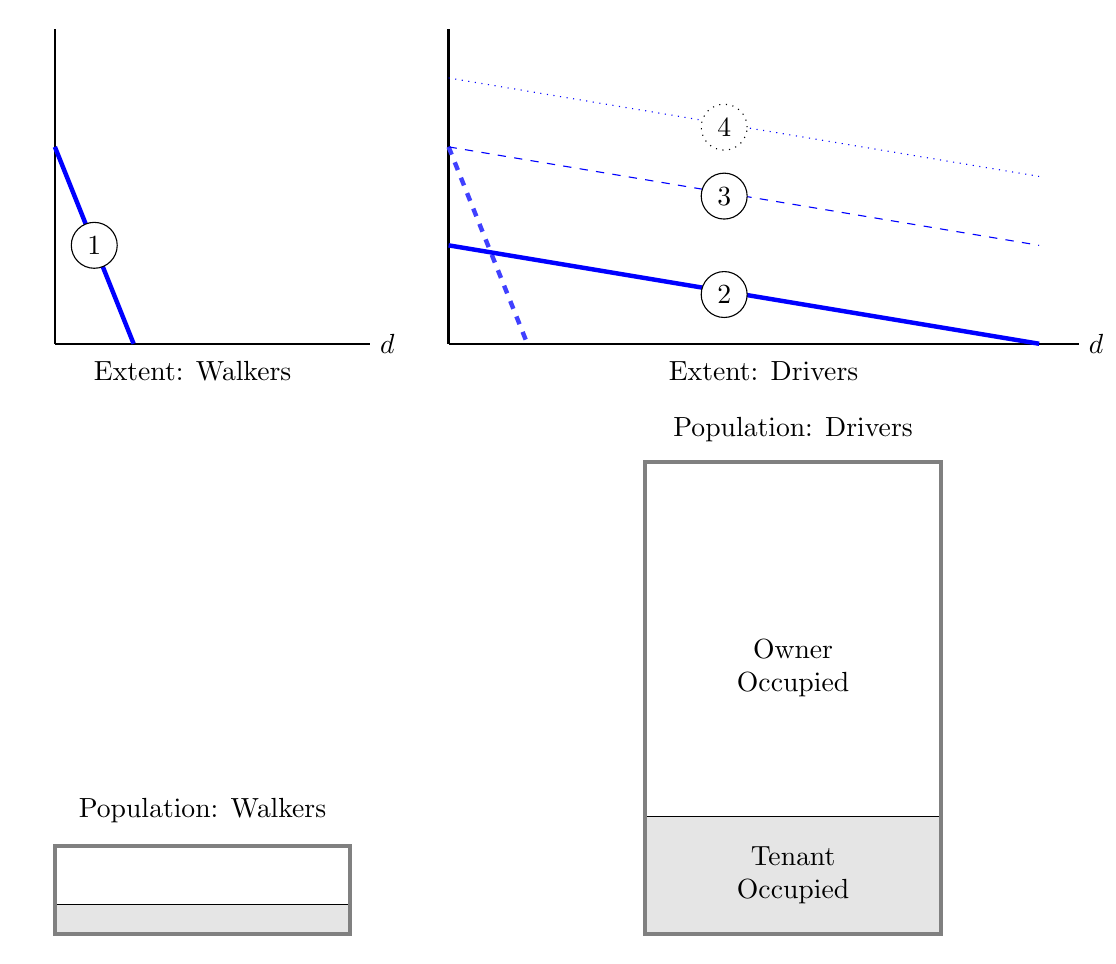
\begin{tikzpicture}[scale=.5]
% EXTENT  BEFORE
\draw[thick](0,0)--(0,8); %Y
\draw[thick](0,0)--(8,0)node[right]{$d$};
\node at (3.5,-.7){Extent: Walkers};
\draw[ultra thick, blue](0,5)--(2,0); 
\node[circle,draw=black, fill=white, inner sep=3pt,minimum size=10pt] (b) at (1,2.5) {1};

% POPULATION BEFORE
\begin{scope}[shift={(0, -15cm)},scale=1.5]%population
\draw [fill=gray!20,] (0,0) rectangle (5,.5); 
\draw[line width= .5mm, black!50] (0,0) rectangle (5,1.5);
\node at (2.5,2.1){Population: Walkers};
\end{scope}

% EXTENT AFTER
\begin{scope}[shift={(10cm, 0)}]
\draw[thick](0,0)--(0,8); %Y
\draw[thick](0,0)--(16,0)node[right]{$d$}; %X
\node at (8,-.7){Extent: Drivers};
\draw[ultra thick, blue!75, dashed](0,5)--(2,0);
\draw[ultra thick, blue](0,2.5)--(15,0);

\node[circle,draw=black, fill=white, inner sep=3pt,minimum size=10pt] (b) at (7,1.25) {2};

\draw[ blue, dashed](0,5)--(15,2.5);
\node[circle,draw=black, fill=white, inner sep=3pt,minimum size=10pt] (b) at (7,3.75) {3};

\draw[ blue, dotted](0,6.75)--(15,4.25);
\node[circle,draw=black, dotted,fill=white, inner sep=3pt,minimum size=10pt] (b) at (7,5.5) {4};
\end{scope}

% POPULATION AFTER
\begin{scope}[shift={(15, -15cm)},scale=1.5]%population
\draw [fill=gray!20,] (0,0) rectangle (5,2); 
\draw[line width= .5mm, black!50] (0,0) rectangle (5,8);
\node at (2.5,8.55){Population: Drivers};
\node at (2.5,4.5)
    [text width=2.4cm, align=center]
    {\baselineskip=20pt Owner Occupied};
%\node at (2,3.3)    [text width=2.4cm]    {\baselineskip=20pt Mortgaged};
\node at (2.5,1)
    [text width=2.4cm, align=center]
    {\baselineskip=20pt Tenant Occupied};
\end{scope}
\label{fig-rent-driving}
\end{tikzpicture}
\caption{Housing tenure post transportation revolution.}
\label{fig-transport-tenure}
\end{figure} 
 
%\input{fig_TransportCost.tex}

The transportation cost revolution brought about by the first street cars and later automobiles made much larger cities possible.  The average walking pace is 2.5 to 4 mph, and new transportation technologies raise this rate by a factor of between five and ten, increasing potential urban area by between twenty-five and one hundred times.   

% THIS IS INTERSTING K.  morgages: Effect of a finbancial instument on urban form!!  suburban flight, second half of the century

%Electric trolleys drew upon manufacturing technology that appeared only in the eighteen eighties and at first only in America. 

%As with other transportation revolutions, institutional as well as technological revolutions were necessary for the interurban phenomenon to succeed.  One such institutional revolution was the creation of the home mortgage in the eighteen eighties.  Another was the development of the public utility, a regulated monopoly, in the earlier twentieth. century.\footnote{https://faculty.washington.edu/jbs/itrans/charge20.htm} The automotive revolution was as important in its way as the coming of the railroads.

%The automobile in time established even more powerful synergies, but they weren't present at the beginning.  Roads suitable for automobiles scarcely existed though new methods of paving utilizing macadam or concrete had recently been invented.  Furthermore, there was no good model in place for road construction.   Unlike the case with either light or heavy rail systems, the vehicles and the road itself were not part of the same corporate entity.       

%Once automotive ownership assumed certain proportions toward the close of the teens of the century, the automobile began to transform the landscape of America in an even more fundamental way than the streetcars had. 

%From the second decade of the twentieth century, the automobile in America has been linked with suburban flight, and when the growth of suburbs reached a crescendo early in the second half of the century, automobile ownership became the norm. 

% Because exurbs are already numerous and growing more so, they place considerable pressure on the Body Politic to ensure that fuel prices remain low, for if prices rise beyond a certain point the exurbanites will be forced to sell out, probably at ruinously low returns because few will choose to live in isolated areas without affordable transportation.  True, exurbs could conceivably be served by public transportation, but only at enormous cost per rider because the population densities are so low in the areas where they are located \dots

% That places the vast suburb dwelling public at risk and the exurbanites most of all.

Initially, rents fell at the centre and rose outside of the original city limits. Lower rents and cheaper suburban housing attract more workers, so that central rents and the land values they support  rise to the original levels and then, because the rising population makes the city more productive, beyond the original level. 

It  also affected social structure and left indelible marks on the form of cities developing at the time and after. In North America, with large amounts of land, it generated massive urban sprawl, but also made land available for a growing `middle class' of homeowners. This homeowning middle class became the dominant social formation in North 
American society. 

Ultimately the urban expansion generated congestion and rising transportation cost that began to limit urban growth, put upward pressure on  housing costs including transportation, and therefore downward pressure on middle-class effective incomes. Rising congestion costs steepen the rent profile and  reduce the net productivity of cities. Although the process is not a focus of this thesis it represents a relatively simple extension for later work.


\section{Municipal costs and revenue}

\begin{figure}
\begin{center}
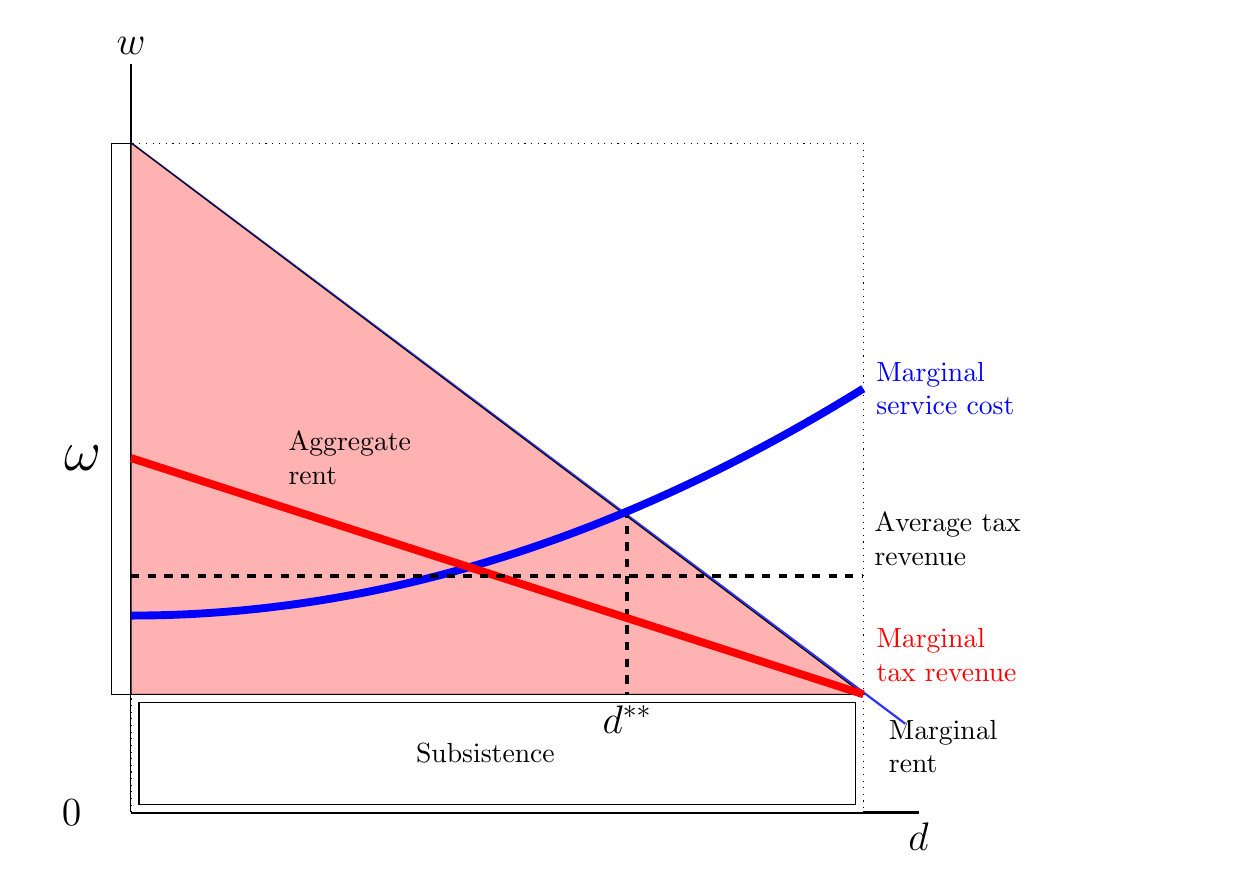
\begin{tikzpicture}[scale=1]
\def\bndmax{5}        %https://tex.stackexchange.com/questions/68462/filling-a-complex-region-with-tikz
\def\bndmin{0.2}
\def \n {8}  % height of y axis
\def \d {10}  % length  of x axis
\def \t {.75}  %  cost of transportation per unit x
\def \th {1}   %
\def \w {7}    %  wage premium
\def \om{1.5}%  omega =rural wage Zero for urban population
\def \azero{2}
\def \aprime {-.0}	
\tikzset{func/.style={thick,color=blue!80}}	
\draw [thick] (0,-\om) --(\d,-\om)node[below]{\Large $d$};  			% Zero for rural population
\draw [thick] (0,-\om)node[left=.5]{\Large $0$} --(0,\n)node[above]{\Large $w$};	% Y axis

%\draw [thick] (0,0)node[left=.5]{ subsistance}--(\d,0);
\node[left=.25] at (0,3){\huge $\omega$};
%\node[left=.25] at (0,\w+.3){subsistence plus};
%\node[left=.25] at (0,\w-.4){wage premium};	

\draw[fill=white, white] (0.1,-0.1) rectangle (14,-\om+.1);
\draw [] (-.25, 0) rectangle(.25, \w);%fill=green!30!blue!30
\node[right] at  (.25, \w/2){Added Productivity};
%\draw [ thick, ->](11.3,-\om/2)--(13, -\om/2)node [right] {\Large $d$};
\draw[fill=blue!40] (0.1,-0.1) rectangle (9.2,-\om+.1);

\draw[fill=black!0, dotted] (0,-\om) rectangle (9.30,\w);% new product repeat
\draw[func, domain=0:\w/\t+.5] plot [samples=200] (\x,{\w-\t*\x}); %rent profile
\draw[fill=blue!0] (0.1,-0.1) rectangle (9.2,-\om+.1);
\node at (4.5,-\om/2){Subsistence};
\draw[fill=red!30,] (0.,0.)--(0,7)--(9.30,0.)--cycle;% Rent \w-.2
\node[text width=2cm] at (3.,3){Aggregate \\rent}; 		%Rent 
%\node at (5.8,5.7)[]{\Large Transportation};
\node at (6.3,4.8)[white]{\Large expenditure};
\draw[ line width=.5mm, dashed] (6.3,2.35)--(6.3,0)node[below ]{\Large $d^{**}$};

\draw[func, domain=0:9.3, line width=1mm,blue, text width=2cm] plot [samples=200] (\x,{1+\x^2/30})node[right]{Marginal\\ service cost};
\draw[ line width=1mm, red] (0,3)--(9.3,0)node[above right, text width=3cm ]{Marginal\\tax revenue};
\node at (9.5, -.2)[below right, text width=2cm]{Marginal rent};

\draw[ line width=.5mm, dashed] (0,1.5)--(9.3,1.5)node[above right, text width=2.5cm ]{Average tax revenue};
%GRID
%\draw[step=1cm,gray,very thin] (0,0) grid (10,10);
\end{tikzpicture}
\end{center}
\caption[The Alonso model with municipal costs and revenue.]{The Alonso model \gls{rent profile}, as illustrated in Figure~\ref{fig-alonso-simple}, with cost and municipal costs and revenue added.} %service fees added.}
\label{fig-municipal-costs}
\end{figure}
 

 Two stylized facts should be noticed. The first is that the marginal cost of servicing generally rises with the distance from the centre. Figure illustrates the general form of servicing costs, but not the relative scales of rent and servicing costs. When this observation is combined with the \gls{Henry George Theorem} the conclusion is that the optimal size of the city  is at  $d^{**}$, where marginal service cost intersects with the marginal increase in total urban rent.  Walter Christaller, 1933

The second stylized fact is that property taxes, which are generally  fixed as a share of property value, decline as the distance from the centre increases. Figure~\ref{fig-municipal-costs} illustrates the general form of tax liabilities, although it does not  accurately represent their relationship to rent or  servicing costs. This implies that in many or most urban situations the residents at the outer edges pay less than the average amount in property tax per unit of land, but cost  the community budget more than the average amount. In essence, the central city subsidizes the suburbs. (see Perverse Cities \ref{blaisPerverseCitiesHidden2011}). This arrangement is both economically inefficient and unfair, but it has been built into the fiscal structure of cities largely as a result of automobile-based urban growth. It is likely that this fiscal misallocation saps some of the potential productivity growth of cities. Property taxation reduces the market value of properties, but it also funds services and amenities that increase the value of properties. 

Both servicing and taxation effects are more variable and than the simple model suggests.  One conclusion urban theorists draw based on variants of the Alonso model is that because property owners in the low-density urban margin are subsidized,  the subsidy is likely to create serious fiscal problems for municipalities in the long-term and result in serious inefficiency in land use.

Political opposition is essentially rent seeking.



\chaptermark{An essay on transsportation}
% Renmoved form old housing Chapter, which was  included in Extensions.
{\color{red}
\section{An essay on transportation costs and the city}
One of the first applications of the model was to the effect of a transportation revolution. The advent of first rail transportation and then the automobile radically changed the size, productivity, and population distribution of cities.
periphery available, allowing larger lot sizes and larger homes for those who can afford them.

\begin{figure}[!hb]
\centering
% CHANGING TRANSPORTATION COSTS
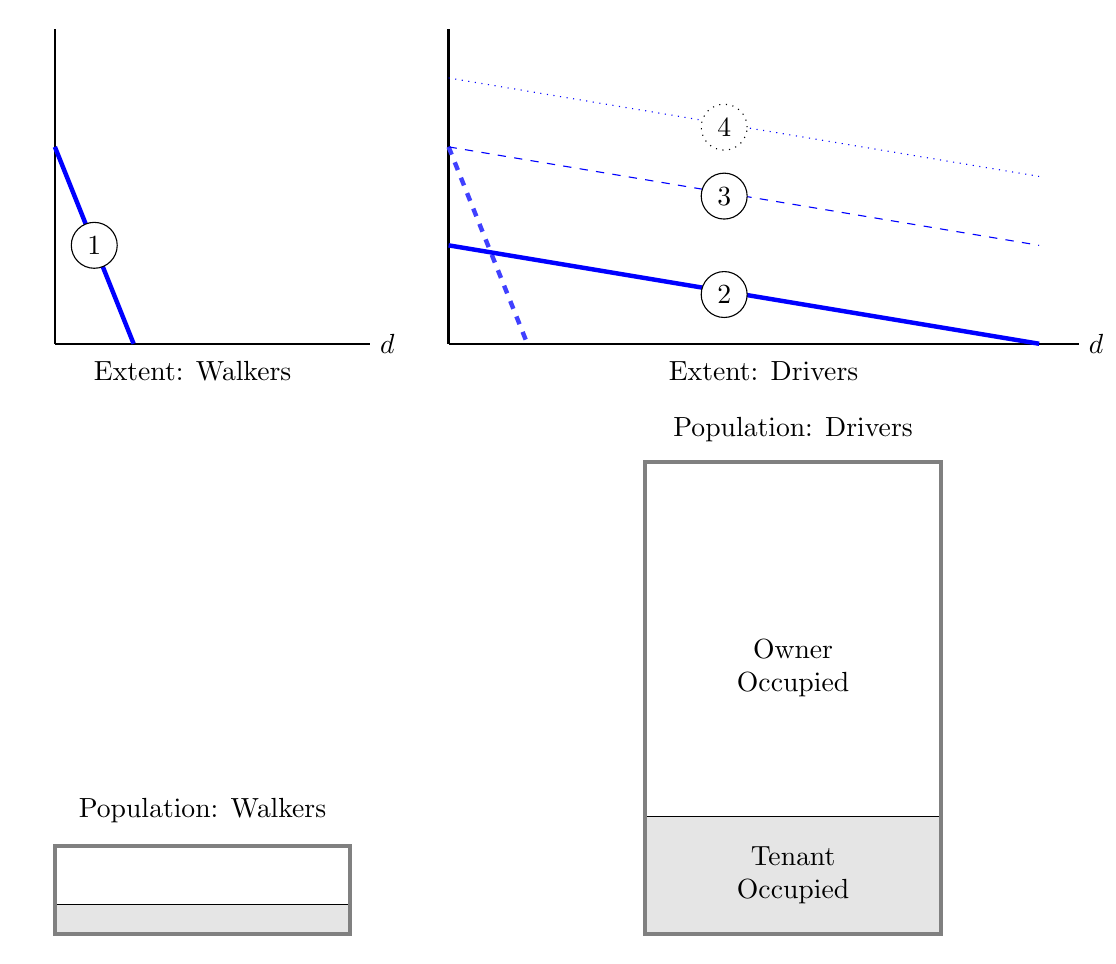
\begin{tikzpicture}[scale=.5]
% EXTENT  BEFORE
\draw[thick](0,0)--(0,8); %Y
\draw[thick](0,0)--(8,0)node[right]{$d$};
\node at (3.5,-.7){Extent: Walkers};
\draw[ultra thick, blue](0,5)--(2,0); 
\node[circle,draw=black, fill=white, inner sep=3pt,minimum size=10pt] (b) at (1,2.5) {1};

% POPULATION BEFORE
\begin{scope}[shift={(0, -15cm)},scale=1.5]%population
\draw [fill=gray!20,] (0,0) rectangle (5,.5); 
\draw[line width= .5mm, black!50] (0,0) rectangle (5,1.5);
\node at (2.5,2.1){Population: Walkers};
\end{scope}

% EXTENT AFTER
\begin{scope}[shift={(10cm, 0)}]
\draw[thick](0,0)--(0,8); %Y
\draw[thick](0,0)--(16,0)node[right]{$d$}; %X
\node at (8,-.7){Extent: Drivers};
\draw[ultra thick, blue!75, dashed](0,5)--(2,0);
\draw[ultra thick, blue](0,2.5)--(15,0);

\node[circle,draw=black, fill=white, inner sep=3pt,minimum size=10pt] (b) at (7,1.25) {2};

\draw[ blue, dashed](0,5)--(15,2.5);
\node[circle,draw=black, fill=white, inner sep=3pt,minimum size=10pt] (b) at (7,3.75) {3};

\draw[ blue, dotted](0,6.75)--(15,4.25);
\node[circle,draw=black, dotted,fill=white, inner sep=3pt,minimum size=10pt] (b) at (7,5.5) {4};
\end{scope}

% POPULATION AFTER
\begin{scope}[shift={(15, -15cm)},scale=1.5]%population
\draw [fill=gray!20,] (0,0) rectangle (5,2); 
\draw[line width= .5mm, black!50] (0,0) rectangle (5,8);
\node at (2.5,8.55){Population: Drivers};
\node at (2.5,4.5)
    [text width=2.4cm, align=center]
    {\baselineskip=20pt Owner Occupied};
%\node at (2,3.3)    [text width=2.4cm]    {\baselineskip=20pt Mortgaged};
\node at (2.5,1)
    [text width=2.4cm, align=center]
    {\baselineskip=20pt Tenant Occupied};
\end{scope}
\label{fig-rent-driving}
\end{tikzpicture}
\caption{Housing tenure post transportation revolution.}
\label{fig-transport-tenure}
\end{figure} 
 
%\input{fig_TransportCost.tex}

The transportation cost revolution brought about by the first street cars and later automobiles made much larger cities possible.  The average walking pace is 2.5 to 4 mph, and new transportation technologies raise this rate by a factor of between five and ten, increasing potential urban area by between twenty-five and one hundred times. 




% THIS IS INTERSTING K.  morgages: Effect of a finbancial instument on urban form!!  suburban flight, second half of the century

%Electric trolleys drew upon manufacturing technology that appeared only in the eighteen eighties and at first only in America. 

%As with other transportation revolutions, institutional as well as technological revolutions were necessary for the interurban phenomenon to succeed.  One such institutional revolution was the creation of the home mortgage in the eighteen eighties.  Another was the development of the public utility, a regulated monopoly, in the earlier twentieth. century.\footnote{https://faculty.washington.edu/jbs/itrans/charge20.htm} The automotive revolution was as important in its way as the coming of the railroads.

%The automobile in time established even more powerful synergies, but they weren't present at the beginning.  Roads suitable for automobiles scarcely existed though new methods of paving utilizing macadam or concrete had recently been invented.  Furthermore, there was no good model in place for road construction.   Unlike the case with either light or heavy rail systems, the vehicles and the road itself were not part of the same corporate entity.       

%Once automotive ownership assumed certain proportions toward the close of the teens of the century, the automobile began to transform the landscape of America in an even more fundamental way than the streetcars had. 

%From the second decade of the twentieth century, the automobile in America has been linked with suburban flight, and when the growth of suburbs reached a crescendo early in the second half of the century, automobile ownership became the norm. 

% Because exurbs are already numerous and growing more so, they place considerable pressure on the Body Politic to ensure that fuel prices remain low, for if prices rise beyond a certain point the exurbanites will be forced to sell out, probably at ruinously low returns because few will choose to live in isolated areas without affordable transportation.  True, exurbs could conceivably be served by public transportation, but only at enormous cost per rider because the population densities are so low in the areas where they are located \dots

% That places the vast suburb dwelling public at risk and the exurbanites most of all.

Initially, rents fell at the centre and rose outside of the original city limits. Lower rents and cheaper suburban housing attract more workers, so that central rents and the land values they support  rise to the original levels and then, because the rising population makes the
city more productive, beyond the original level. 

It  also affected social structure and left indelible marks on the form of cities developing at the time and after. In North America, with large amounts of land, it generated massive urban sprawl, but also made land available for a growing `middle class' of homeowners. This homeowning middle class became the dominant social formation in North 
American society. 

Ultimately the urban expansion generated congestion and rising transportation cost that began to limit urban growth, put upward pressure on  housing costs including transportation, and therefore downward pressure on middle-class effective incomes. Rising congestion costs steepen the rent profile and  reduce the net productivity of cities. Although the process is not a focus of this thesis it represents a relatively simple extension for later work.

\subsection{Differential transportation costs}
 Urbanists agree that before the railroad and the automobile, the extent of a city was roughly determined by how far a person could walk in about an hour. The time and effort cost of transportation determined the size of cities. 
 
 It also affected the distribution of the classes within the city. When everyone walked, the  wealthy may have valued their time more than the poor. In terms of the model, the willingness to pay of the rich would higher  near the core than  the willingness (or ability) to pay of  the poor, but would descend more rapidly with distance
\begin{figure}
\begin{center}
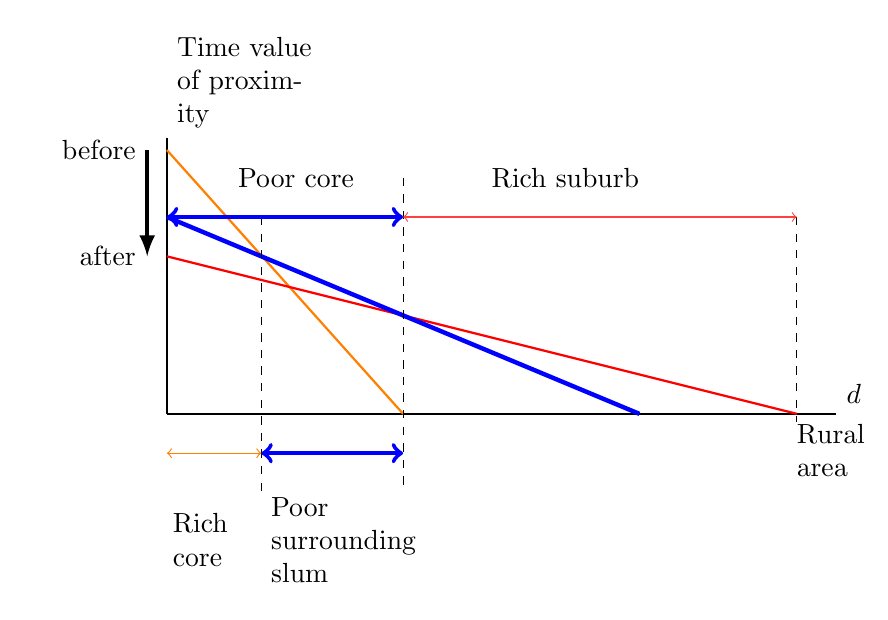
\begin{tikzpicture}[scale=1]
% AXES
\draw[thick](0,0)--(0,3.5)node[above right, text width=1.8cm]{Time  value of proximity}; %Y++
\draw[thick](0,0)--(8.5,0)node[above right]{$d$}node[below, text width =1cm]{Rural area}; 
% BIDS-RENT CURVES
\draw[thick, orange](0,3.35)--(3,0);
\draw[thick, red](0,2)--(8,0);
\draw[ultra thick, blue](0,2.5)--(6,0);

\draw[-latex, ultra thick](-.25,3.35)node[left]{before}--(-.25,2)node[left]{after};
% ZONE DIVISIONS VERTICAL LINES
\draw[dashed](1.2,2.5)--(1.2,-1) ;
\draw[dashed](3,3)--(3,-1) ;
\node at (4,3)[right]{Rich suburb};
\node at (2.5,3)[left]{Poor core};
\draw[dashed](8,2.5)--(8,-.1) ;
%  ARROWS BEFORE
\draw[<->, orange](0,-.5)--(1.2,-.5);
\draw[<->, blue, ultra thick](3,-.5)--(1.2,-.5);
\node[text width =1cm,  left] at (1.2,-1.6){Rich core };
\node[text width =1cm, right] at (1.2,-1.6){Poor \\ surrounding slum};
%  ARROWS AFTER
\draw[<->, blue, ultra thick](0,2.5)--(3,2.5);
\draw[<->, red!75](3,2.5)--(8,2.5);

% \draw[ blue, dashed](0,5)--(15,2.5);
% \node[circle,draw=black, fill=white, inner sep=3pt,minimum size=10pt] (b) at (7,3.75) {3};

% \draw[ blue, dotted](0,6.75)--(15,4.25);
% \node[circle,draw=black, dotted,fill=white, inner sep=3pt,minimum size=10pt] (b) at (7,5.5) {4};
\end{tikzpicture}\end{center}
\caption{A prediction of the basic model: if transportation cost for the rich falls, shifting the orange  bid-rent curve for the rich to the location of the red line, we will see a shift of housing for the rich  from the core to the suburb.}
% \label{fig_fix_my_label}
\end{figure}

 If the technology suddenly provides the rich with commuter trains or automobiles and more attractive sites at the edge of the city, the orange line could drop enough  and become much flatter leading in a flight of the rich to the suburbs, as appears to have happened in many American cities. Lower transportation costs make cheaper land on the edge of the city attractive. This would  offer  more space and the opportunity to build larger homes, a pattern that has emerged in some cities.

\textbf{Experiments}: We first turn off financial  demand and partition the population by wealth and transportation cost to  verify that the predictions made by researchers hold in our model. We then turn financial demand back on  and see if the rate or degree of financialization differs from the base model


\subsection{Municipal costs and revenue}

\begin{figure}
\begin{center}
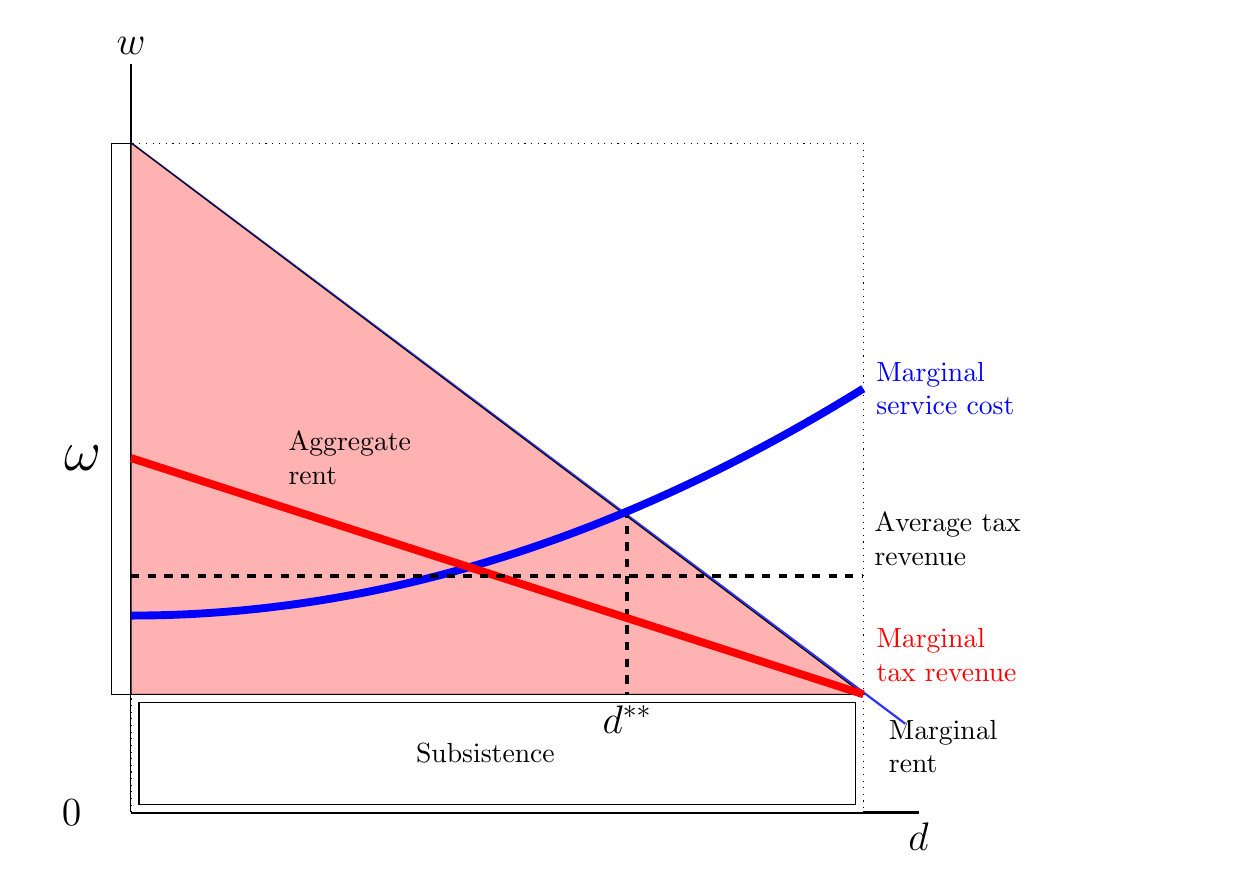
\begin{tikzpicture}[scale=1]
\def\bndmax{5}        %https://tex.stackexchange.com/questions/68462/filling-a-complex-region-with-tikz
\def\bndmin{0.2}
\def \n {8}  % height of y axis
\def \d {10}  % length  of x axis
\def \t {.75}  %  cost of transportation per unit x
\def \th {1}   %
\def \w {7}    %  wage premium
\def \om{1.5}%  omega =rural wage Zero for urban population
\def \azero{2}
\def \aprime {-.0}	
\tikzset{func/.style={thick,color=blue!80}}	
\draw [thick] (0,-\om) --(\d,-\om)node[below]{\Large $d$};  			% Zero for rural population
\draw [thick] (0,-\om)node[left=.5]{\Large $0$} --(0,\n)node[above]{\Large $w$};	% Y axis

%\draw [thick] (0,0)node[left=.5]{ subsistance}--(\d,0);
\node[left=.25] at (0,3){\huge $\omega$};
%\node[left=.25] at (0,\w+.3){subsistence plus};
%\node[left=.25] at (0,\w-.4){wage premium};	

\draw[fill=white, white] (0.1,-0.1) rectangle (14,-\om+.1);
\draw [] (-.25, 0) rectangle(.25, \w);%fill=green!30!blue!30
\node[right] at  (.25, \w/2){Added Productivity};
%\draw [ thick, ->](11.3,-\om/2)--(13, -\om/2)node [right] {\Large $d$};
\draw[fill=blue!40] (0.1,-0.1) rectangle (9.2,-\om+.1);

\draw[fill=black!0, dotted] (0,-\om) rectangle (9.30,\w);% new product repeat
\draw[func, domain=0:\w/\t+.5] plot [samples=200] (\x,{\w-\t*\x}); %rent profile
\draw[fill=blue!0] (0.1,-0.1) rectangle (9.2,-\om+.1);
\node at (4.5,-\om/2){Subsistence};
\draw[fill=red!30,] (0.,0.)--(0,7)--(9.30,0.)--cycle;% Rent \w-.2
\node[text width=2cm] at (3.,3){Aggregate \\rent}; 		%Rent 
%\node at (5.8,5.7)[]{\Large Transportation};
\node at (6.3,4.8)[white]{\Large expenditure};
\draw[ line width=.5mm, dashed] (6.3,2.35)--(6.3,0)node[below ]{\Large $d^{**}$};

\draw[func, domain=0:9.3, line width=1mm,blue, text width=2cm] plot [samples=200] (\x,{1+\x^2/30})node[right]{Marginal\\ service cost};
\draw[ line width=1mm, red] (0,3)--(9.3,0)node[above right, text width=3cm ]{Marginal\\tax revenue};
\node at (9.5, -.2)[below right, text width=2cm]{Marginal rent};

\draw[ line width=.5mm, dashed] (0,1.5)--(9.3,1.5)node[above right, text width=2.5cm ]{Average tax revenue};
%GRID
%\draw[step=1cm,gray,very thin] (0,0) grid (10,10);
\end{tikzpicture}
\end{center}
\caption[The Alonso model with municipal costs and revenue.]{The Alonso model \gls{rent profile}, as illustrated in Figure~\ref{fig-alonso-simple}, with cost and municipal costs and revenue added.} %service fees added.}
\label{fig-municipal-costs}
\end{figure}
 

 Two stylized facts should be noticed. The first is that the marginal cost of servicing generally rises with the distance from the centre. Figure illustrates the general form of servicing costs, but not the relative scales of rent and servicing costs. When this observation is combined with the \gls{Henry George Theorem} the conclusion is that the optimal size of the city  is at  $d^{**}$, where marginal service cost intersects with the marginal increase in total urban rent.  Walter Christaller, 1933

The second stylized fact is that property taxes, which are generally  fixed as a share of property value, decline as the distance from the centre increases. Figure~\ref{fig-municipal-costs} illustrates the general form of tax liabilities, although it does not  accurately represent their relationship to rent or  servicing costs. This implies that in many or most urban situations the residents at the outer edges pay less than the average amount in property tax per unit of land, but cost  the community budget more than the average amount. In essence, the central city subsidizes the suburbs. (see Perverse Cities \ref{blaisPerverseCitiesHidden2011}). This arrangement is both economically inefficient and unfair, but it has been built into the fiscal structure of cities largely as a result of automobile-based urban growth. It is likely that this fiscal misallocation saps some of the potential productivity growth of cities. Property taxation reduces the market value of properties, but it also funds services and amenities that increase the value of properties. 

Both servicing and taxation effects are more variable and than the simple model suggests.  One conclusion urban theorists draw based on variants of the Alonso model is that because property owners in the low-density urban margin are subsidized,  the subsidy is likely to create serious fiscal problems for municipalities in the long-term and result in serious inefficiency in land use.

Political opposition is essentially rent seeking.

}
\end{document}